\documentclass[conference]{IEEEtran}
\IEEEoverridecommandlockouts

\usepackage{cite}
\usepackage{amsmath,amssymb,amsfonts}
\usepackage{algorithmic}
\usepackage{graphicx}
\graphicspath{{figures/}{./}}
\usepackage{textcomp}
\usepackage{xcolor}
\usepackage{booktabs}
\usepackage{multirow}
\usepackage{url}
\usepackage{hyperref}

\def\BibTeX{{\rm B\kern-.05em{\sc i\kern-.025em b}\kern-.08em
    T\kern-.1667em\lower.7ex\hbox{E}\kern-.125emX}}

\begin{document}

\title{Spatio-Temporal Air Quality Prediction in Indian Urban Environments: Numerical Forecasting Benchmarks, Image-Based Estimation, and Multimodal Alignment Feasibility}

\author{
\IEEEauthorblockN{Teliki Rushya Sree\IEEEauthorrefmark{1}, Machireddy Swathi\IEEEauthorrefmark{1}, Thanuja Varakala\IEEEauthorrefmark{1}, Palli Shilpa\IEEEauthorrefmark{1}, and Thotta Ramatulasi\IEEEauthorrefmark{2}}
\IEEEauthorblockA{\IEEEauthorrefmark{1}Department of Computer Science and Engineering\\
\IEEEauthorrefmark{2}Faculty Supervisor\\
[Affiliation Placeholder: University / Engineering Institution Name, City, State, India]\\
[Email Placeholder: \{rushyasree.t, swathi.m, thanuja.v, shilpa.p, ramatulasi.t\}@institution.edu]}
}

\maketitle

\begin{abstract}
Urban air pollution across Indian metropolitan areas poses severe environmental and public health hazards, driven by elevated concentrations of fine ($\text{PM}_{2.5}$) and coarse ($\text{PM}_{10}$) particulate matter. While deep learning has proven effective for numerical time-series forecasting, recent literature has increasingly proposed multimodal architectures that fuse ground telemetry with outdoor camera imagery. In this work, we conduct a rigorous empirical investigation of spatio-temporal air quality prediction across 90 Central Pollution Control Board (CPCB) monitoring stations spanning 2015--2020 integrated with ERA5-Land reanalysis meteorology and outdoor environmental imagery from PM25Vision. We evaluate: (i) an operational-scale numerical Long Short-Term Memory (LSTM) forecaster on 1,369,779 hourly records predicting next-hour concentrations ($t+1$), achieving a test $\text{PM}_{2.5}$ Mean Absolute Error (MAE) of 10.5719 $\mu\text{g/m}^3$ ($R^2 = 0.9492$) and $\text{PM}_{10}$ MAE of 18.8643 $\mu\text{g/m}^3$ ($R^2 = 0.9301$) on 404,431 held-out sequences, outperforming persistence baselines; and (ii) an image-only transfer learning model based on ResNet-50 evaluated on 640 unique, deduplicated outdoor images across India, achieving test $\text{PM}_{2.5}$ MAE of 66.2148 $\mu\text{g/m}^3$ ($R^2 = 0.1524$) across 18 held-out spatial-temporal groups. Furthermore, we conduct a comprehensive feasibility audit on multimodal fusion. We demonstrate that combining opportunistic web-scraped imagery with continuous hourly telemetry is scientifically indefensible due to: (a) absence of sub-daily image timestamps, despite an average intraday station $\text{PM}_{2.5}$ swing of 166.72 $\mu\text{g/m}^3$; (b) an effective sample size of only 36 independent station-date groups within a 5 km radius, with 40\% of images concentrated in just two single-day bursts; and (c) a systematic positive image-to-station label bias of $+70.74\ \mu\text{g/m}^3$. A controlled exploratory fusion experiment on the matched cohort ($N=60$ test instances across 9 independent groups) reveals that early feature fusion degrades out-of-distribution generalization compared to image-only models ($\text{PM}_{2.5}$ MAE 85.86 vs. 73.67 $\mu\text{g/m}^3$; $R^2 = -0.5064$ vs. $-0.2070$). We conclude by outlining essential requirements for viable future multimodal air quality forecasting networks.
\end{abstract}

\begin{IEEEkeywords}
Air Quality Forecasting, PM2.5, PM10, Deep Learning, LSTM, Convolutional Neural Networks, Multimodal Alignment, Spatio-Temporal Modeling, ERA5-Land.
\end{IEEEkeywords}

\section{Introduction}
Severe ambient particulate matter pollution ($\text{PM}_{2.5}$ and $\text{PM}_{10}$) in Indian urban environments represents one of the foremost environmental health crises globally, contributing to elevated respiratory morbidity, cardiovascular mortality, and economic degradation \cite{cpcb2009naaqs}. The complex spatio-temporal dynamics of urban air pollutants are governed by local anthropogenic emissions (vehicular traffic, industrial exhaust, biomass combustion, and construction dust) combined with regional meteorological conditions such as boundary layer height, temperature inversions, relative humidity, and wind dispersion \cite{munoz2021era5land}.

Accurate short-term forecasting is vital for municipal early-warning systems, traffic advisories, and targeted pollution mitigation policies. Traditional atmospheric chemical transport models (CTMs) rely on emission inventories that are frequently outdated or coarse in resolution across developing countries. Consequently, data-driven machine learning and deep recurrent architectures, notably Long Short-Term Memory (LSTM) networks, have emerged as strong predictive approaches by learning non-linear temporal dependencies from continuous automated sensor feeds \cite{hochreiter1997lstm, zheng2015forecasting}.

Concurrently, computer vision researchers have explored estimating particulate matter concentrations directly from outdoor digital images by measuring visual transmission loss, atmospheric haze, and contrast attenuation \cite{liu2016particle, he2016resnet}. A compelling research hypothesis has therefore emerged: \textit{Can optical features extracted from outdoor images be fused with numerical ground sensor feeds and meteorological reanalysis to produce superior multimodal air quality forecasts?}

In this paper, we address this question through an end-to-end empirical study deployed on real-world Indian data. We systematically audit three distinct modeling paradigms:
\begin{enumerate}
    \item \textbf{High-Frequency Numerical Forecasting}: An operational LSTM network trained on 1.37 million hourly records from 90 CPCB continuous stations paired with hourly ERA5-Land meteorological variables.
    \item \textbf{Image-Only Environmental Vision}: A transfer-learning ResNet-50 regression baseline trained on curated outdoor imagery from the PM25Vision dataset across Indian coordinates.
    \item \textbf{Multimodal Alignment \& Feasibility Analysis}: A quantitative audit of spatial, temporal, and distribution alignment between ground sensors and image captures, followed by a controlled exploratory fusion experiment.
\end{enumerate}

Rather than claiming unverified performance gains, we provide an objective analysis of multimodal fusion viability. We demonstrate why naive integration of opportunistic web-sourced images with high-frequency continuous station sequences fails both statistically and methodologically, establishing critical boundary conditions for future multimodal sensing architectures.

\section{Related Work}

\subsection{Numerical Air Quality Time-Series Forecasting}
Data-driven time-series forecasting has evolved from autoregressive integrated moving average (ARIMA) and support vector regression (SVR) to deep recurrent and attention networks. Zheng et al. \cite{zheng2015forecasting} demonstrated that integrating spatial meteorological data with historical air quality measurements significantly improves urban pollution forecasting. Recurrent neural networks, specifically LSTMs \cite{hochreiter1997lstm}, have been widely adopted due to their gating mechanisms that mitigate vanishing gradients over multi-hour lag sequences. Reanalysis products such as ERA5 and ERA5-Land \cite{hersbach2020era5, munoz2021era5land} provide spatially continuous atmospheric variables (temperature, boundary layer dynamics, wind vectors, and humidity) that correlate strongly with pollutant accumulation and dispersion.

\subsection{Image-Based Particulate Matter Estimation}
Visual air quality estimation relies on physical atmospheric optics, where aerosol scattering attenuates light propagation in accordance with the Beer-Lambert law \cite{liu2016particle}. Modern deep convolutional neural networks (CNNs), such as ResNet-50 \cite{he2016resnet}, extract high-level semantic haze and contrast features without hand-crafted dark-channel priors. Large-scale image collections such as PM25Vision \cite{pm25vision2023} have aggregated web-scraped and user-uploaded outdoor images paired with regional air quality labels to benchmark vision-based PM estimation. However, the degree to which image-derived estimates can be meaningfully synchronized with ground monitor time-series remains largely unexamined.

\section{Datasets and Preprocessing}

\subsection{Ground-Station Air Quality (CPCB)}
Historical ground measurements were obtained from the Central Pollution Control Board (CPCB) monitoring network in India covering the period from January 1, 2015 to July 1, 2020 \cite{rao2020cpcbdata}. The raw dataset comprises 90 continuous ambient air quality monitoring stations (CAAQMS) situated across 23 states and union territories. Following quality control, negative concentrations, sensor dropouts, and non-physical values were removed. The cleaned hourly dataset consists of 1,369,779 valid hourly records containing hourly $\text{PM}_{2.5}$ and $\text{PM}_{10}$ targets alongside co-pollutants ($\text{NO}$, $\text{NO}_2$, $\text{NO}_x$, $\text{CO}$, $\text{SO}_2$, $\text{O}_3$).

\subsection{ERA5-Land Meteorological Reanalysis}
Because ground stations frequently lack collocated weather instrumentation, hourly meteorological variables were extracted from the Copernicus Climate Change Service ERA5-Land reanalysis dataset \cite{munoz2021era5land} at a spatial resolution of $0.1^\circ \times 0.1^\circ$ ($\sim 9\text{ km}$). Six atmospheric variables were bilinearly interpolated to the exact latitude and longitude of each of the 90 CPCB stations: 2-meter air temperature ($T$), 2-meter dewpoint temperature ($T_d$), relative humidity ($RH$), 10-meter eastward ($u$) and northward ($v$) wind velocity components, and total precipitation ($P$). Timestamp and station-level merging was 100\% complete across all 1,369,779 rows, as audited in project verification logs.

\subsection{PM25Vision Image Dataset Curation}
Outdoor imagery was sourced from the PM25Vision dataset \cite{pm25vision2023}. A geographic bounding box filter over India ($6^\circ\text{N}$--$38^\circ\text{N}$, $68^\circ\text{E}$--$98^\circ\text{E}$) identified 642 candidate rows. 

To prevent data corruption and evaluation leakage:
\begin{enumerate}
    \item All 642 image files were downloaded and physically verified for readability using PIL; zero files were missing or unreadable.
    \item Exact bit-level duplicate detection using SHA-256 cryptographic hashing identified 2 duplicate files, which were excluded from the modeling manifest while preserving raw files on disk.
    \item The final clean image dataset contains exactly 640 unique physical images and 640 unique image identifiers spanning dates from September 6, 2015 to February 29, 2020.
\end{enumerate}

\section{Numerical Time-Series Forecasting}

\subsection{Sequence Formulation}
To forecast air pollution for operational decision-making, we formulate next-hour prediction as a supervised sliding-window sequence regression problem. Given a 24-hour historical window of observed pollution, meteorology, cyclical time features, and station spatial coordinates:
\begin{equation}
\mathbf{X}_t = [\mathbf{x}_{t-23}, \mathbf{x}_{t-22}, \dots, \mathbf{x}_t] \in \mathbb{R}^{24 \times D}
\end{equation}
the model predicts the pollutant concentrations at the subsequent hour:
\begin{equation}
\hat{\mathbf{y}}_{t+1} = [\widehat{\text{PM}}_{2.5}, \widehat{\text{PM}}_{10}] \in \mathbb{R}^2
\end{equation}
where $D$ represents the input feature dimension comprising 12 pollutant and meteorological variables, cyclical temporal encodings ($\sin/\cos$ of hour and month), and station coordinates.

\subsection{Chronological Partitioning \& Leakage Prevention}
To simulate true operational forecasting and prevent future-lookahead leakage, the 1.37M-record sequence index was partitioned strictly by calendar time:
\begin{itemize}
    \item \textbf{Training Set}: 2015-01-01 to 2018-06-30 (336,641 sequences)
    \item \textbf{Validation Set}: 2018-07-01 to 2019-06-30 (326,423 sequences)
    \item \textbf{Test Set}: 2019-07-01 to 2020-07-01 (404,431 sequences)
\end{itemize}
Standardization (mean and standard deviation) was fitted exclusively on the training partition and applied out-of-sample to validation and test sequences.

\subsection{Network Architecture \& Training}
The forecasting architecture employs a 2-layer LSTM with 64 hidden units per layer, dropout ($p=0.2$), followed by a multi-layer perceptron (MLP) regression head ($64 \rightarrow 64 \rightarrow 2$). The network was trained using the Adam optimizer (learning rate $10^{-3}$, batch size 256) minimizing Mean Squared Error (MSE), with learning rate decay upon validation plateau and early stopping (patience = 5 epochs).

\section{Image-Only CNN Regression Baseline}

\subsection{Architecture \& Feature Extraction}
For standalone visual air quality estimation, we utilize a deep convolutional backbone based on ResNet-50 \cite{he2016resnet} initialized with ImageNet-1K pretrained weights. The final 1000-way classification layer is removed, yielding a 2048-dimensional global average pooled visual feature vector $\mathbf{v}_i \in \mathbb{R}^{2048}$. An MLP regression head is appended:
\begin{equation}
\hat{y}_i = \mathbf{W}_3 \operatorname{ReLU}(\mathbf{W}_2 \operatorname{Dropout}(\operatorname{ReLU}(\operatorname{BN}(\mathbf{W}_1 \mathbf{v}_i))))
\end{equation}
mapping $\mathbb{R}^{2048} \rightarrow \mathbb{R}^{256} \rightarrow \mathbb{R}^{64} \rightarrow \mathbb{R}^1$ to predict continuous $\text{PM}_{2.5}$ concentration ($\mu\text{g/m}^3$).

\subsection{Leakage-Safe Group Partitioning}
Images captured in spatial or temporal proximity often share near-identical background visual features (e.g., street scenes or horizons). Random splitting would cause severe data leakage. We therefore implement a two-stage \texttt{GroupShuffleSplit} grouped on spatial-temporal clusters:
\begin{equation}
\text{group}_i = \text{nearest\_station}_i \,\|\, \text{date}_i
\end{equation}
Across all 640 images, 90 distinct station-date groups exist:
\begin{itemize}
    \item \textbf{Train}: 439 images across 57 groups (30 stations; $\text{PM}_{2.5}$ mean $204.2\ \mu\text{g/m}^3$, range $[21, 445]$)
    \item \textbf{Validation}: 122 images across 15 groups (13 stations; $\text{PM}_{2.5}$ mean $309.2\ \mu\text{g/m}^3$, range $[97, 394]$)
    \item \textbf{Test}: 79 images across 18 groups (13 stations; $\text{PM}_{2.5}$ mean $230.7\ \mu\text{g/m}^3$, range $[64, 461]$)
\end{itemize}
We formally verified that group sets and SHA-256 hashes are strictly disjoint across train, validation, and test splits. Target standardization parameters ($\mu = 204.15$, $\sigma = 61.38\ \mu\text{g/m}^3$) were computed on the training partition only. The model was trained using Smooth L1 Loss with validation checkpoint selection at Epoch 8.

\section{Spatial and Temporal Alignment Feasibility Audit}

Before implementing multimodal fusion, we conducted an empirical audit of the spatial and temporal compatibility between PM25Vision images and CPCB sensor streams.

\subsection{Spatial Proximity Analysis}
Using the vectorized Haversine formula, each image coordinate $(\phi_{\text{img}}, \lambda_{\text{img}})$ was mapped to its nearest station among the 90 CPCB monitors. As illustrated in Fig.~\ref{fig:alignment}(a), distances range from 0.052 km to 620.77 km (median: 5.16 km; mean: 92.78 km). Applying an explicit 5.0 km threshold reveals that:
\begin{itemize}
    \item 316 images (49.4\%) are located within 5 km of a monitor.
    \item 324 images (50.6\%) exceed 5 km and cannot be associated with any ground monitor.
\end{itemize}

\begin{figure}[t]
\centering
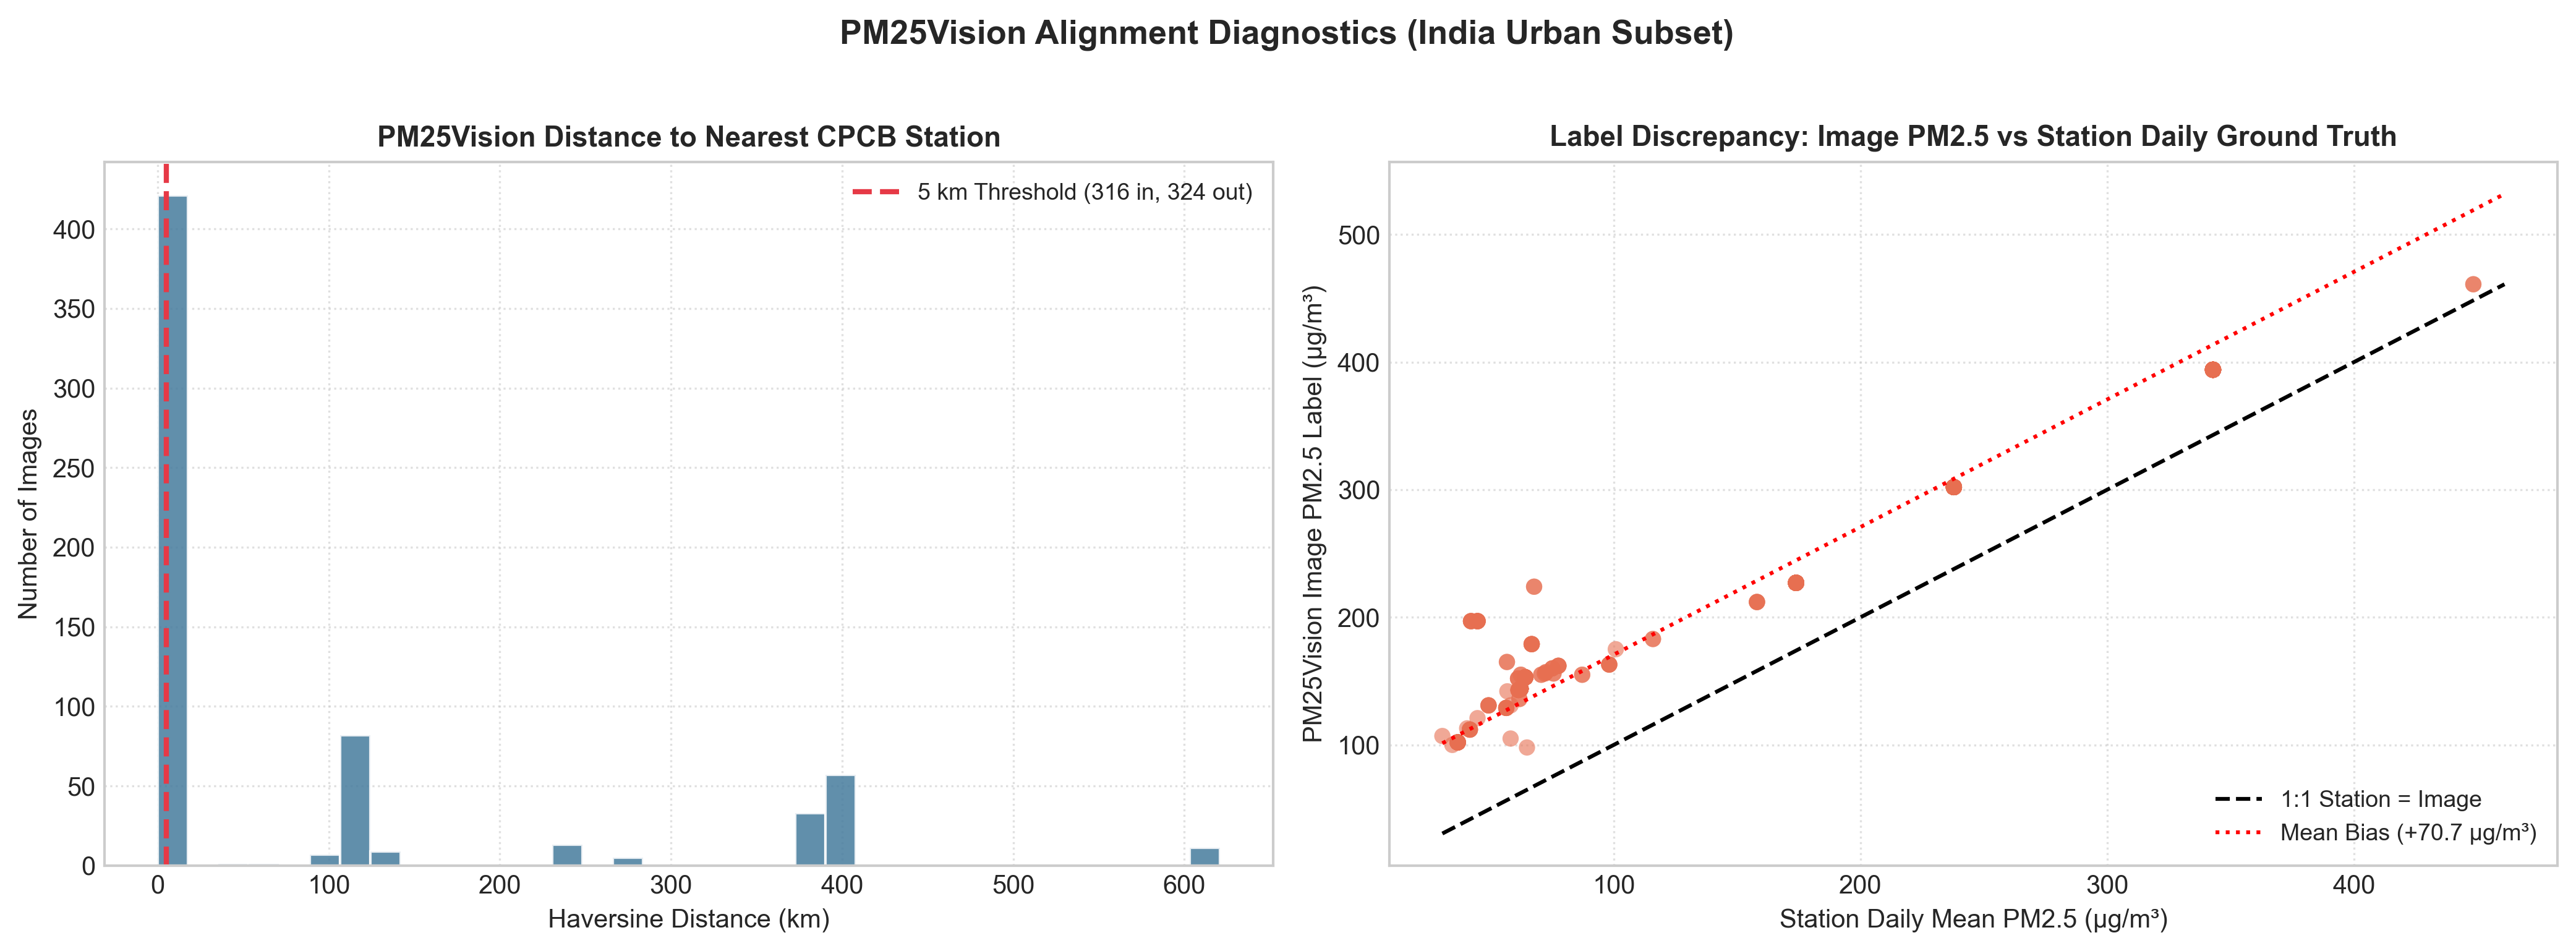
\includegraphics[width=\columnwidth]{alignment_discrepancy_distribution.png}
\caption{PM25Vision alignment diagnostics: (a) Haversine distance distribution to nearest CPCB station; (b) Systematic discrepancy between PM25Vision image labels and collocated station daily ground truth.}
\label{fig:alignment}
\end{figure}

\subsection{Temporal Resolution Mismatch}
The PM25Vision dataset provides only calendar date strings (\texttt{YYYY-MM-DD}) with zero sub-daily hour or minute metadata. At collocated CPCB monitors, ground-truth $\text{PM}_{2.5}$ fluctuates substantially throughout the day due to rush-hour emissions and boundary layer height variations. Across the matched dates, the average intraday station minimum $\text{PM}_{2.5}$ is $85.21\ \mu\text{g/m}^3$, while the average maximum is $251.93\ \mu\text{g/m}^3$, representing an average diurnal range of \textbf{166.72 $\mu\text{g/m}^3$}. Splicing an undated snapshot into a 24-hour sequence or attempting to predict a specific next hour ($t+1$) is mathematically undefined.

\subsection{Sample Size Bottleneck and Burst Clustering}
Of the 316 images within 5 km, exactly 265 images share a calendar date with an active monitor. However, these 265 images represent only \textbf{36 independent station-date groups} across 19 stations over the entire 5.5-year observation period. Furthermore, extreme burst sampling exists:
\begin{itemize}
    \item Station \texttt{DL002} on 2016-01-30 contains 63 images (all labeled with the exact static value $394.0\ \mu\text{g/m}^3$).
    \item Station \texttt{DL026} on 2018-10-24 contains 42 images (all labeled with $227.0\ \mu\text{g/m}^3$).
\end{itemize}
These two single-day events account for 39.6\% of the entire matched dataset. An independent test partition reserving 25\% of groups contains only 9 independent station-date events.

\subsection{Systematic Label Discrepancy}
As shown in Fig.~\ref{fig:alignment}(b), PM25Vision labels average $236.83\ \mu\text{g/m}^3$ across matched pairs, whereas actual station daily ground truth averages $166.09\ \mu\text{g/m}^3$. The mean signed difference ($\text{PM}_{\text{img}} - \text{PM}_{\text{station}}$) is $+70.74\ \mu\text{g/m}^3$ ($\text{MAE} = 70.74\ \mu\text{g/m}^3$). This indicates that image labels reflect distinct calibration standards or localized micro-climates that diverge from certified CAAQMS beta-attenuation monitors.

\section{Controlled Exploratory Fusion Experiment}

To test the empirical effect of combining visual and numerical modalities within the constraints of available data, we conducted a controlled exploratory experiment on the 265 matched records ($N_{\text{groups}}=36$).

\subsection{Experimental Design}
To ensure rigorous evaluation without cross-split leakage, we partitioned the 36 groups using \texttt{GroupShuffleSplit} (seed = 42):
\begin{itemize}
    \item \textbf{Training Partition}: 205 samples across 27 independent station-date groups.
    \item \textbf{Test Partition}: 60 samples across 9 held-out station-date groups (mean station $\text{PM}_{2.5} = 131.7\ \mu\text{g/m}^3$, $\sigma = 86.8\ \mu\text{g/m}^3$).
\end{itemize}

Three models were fitted on the training split and evaluated on the \textbf{exact same 60 test instances}:
\begin{enumerate}
    \item \textbf{Numerical-Only}: Ridge regression on daily ERA5-Land weather features ($T, T_d, RH, \text{wind speed}, P$).
    \item \textbf{Image-Only}: Ridge regression on 2048-dim ResNet-50 embeddings.
    \item \textbf{Multimodal Early Fusion}: Ridge regression on concatenated normalized visual and meteorological vectors ($[\mathbf{v}_i, \mathbf{w}_i] \in \mathbb{R}^{2053}$).
\end{enumerate}

\begin{figure*}[t]
\centering
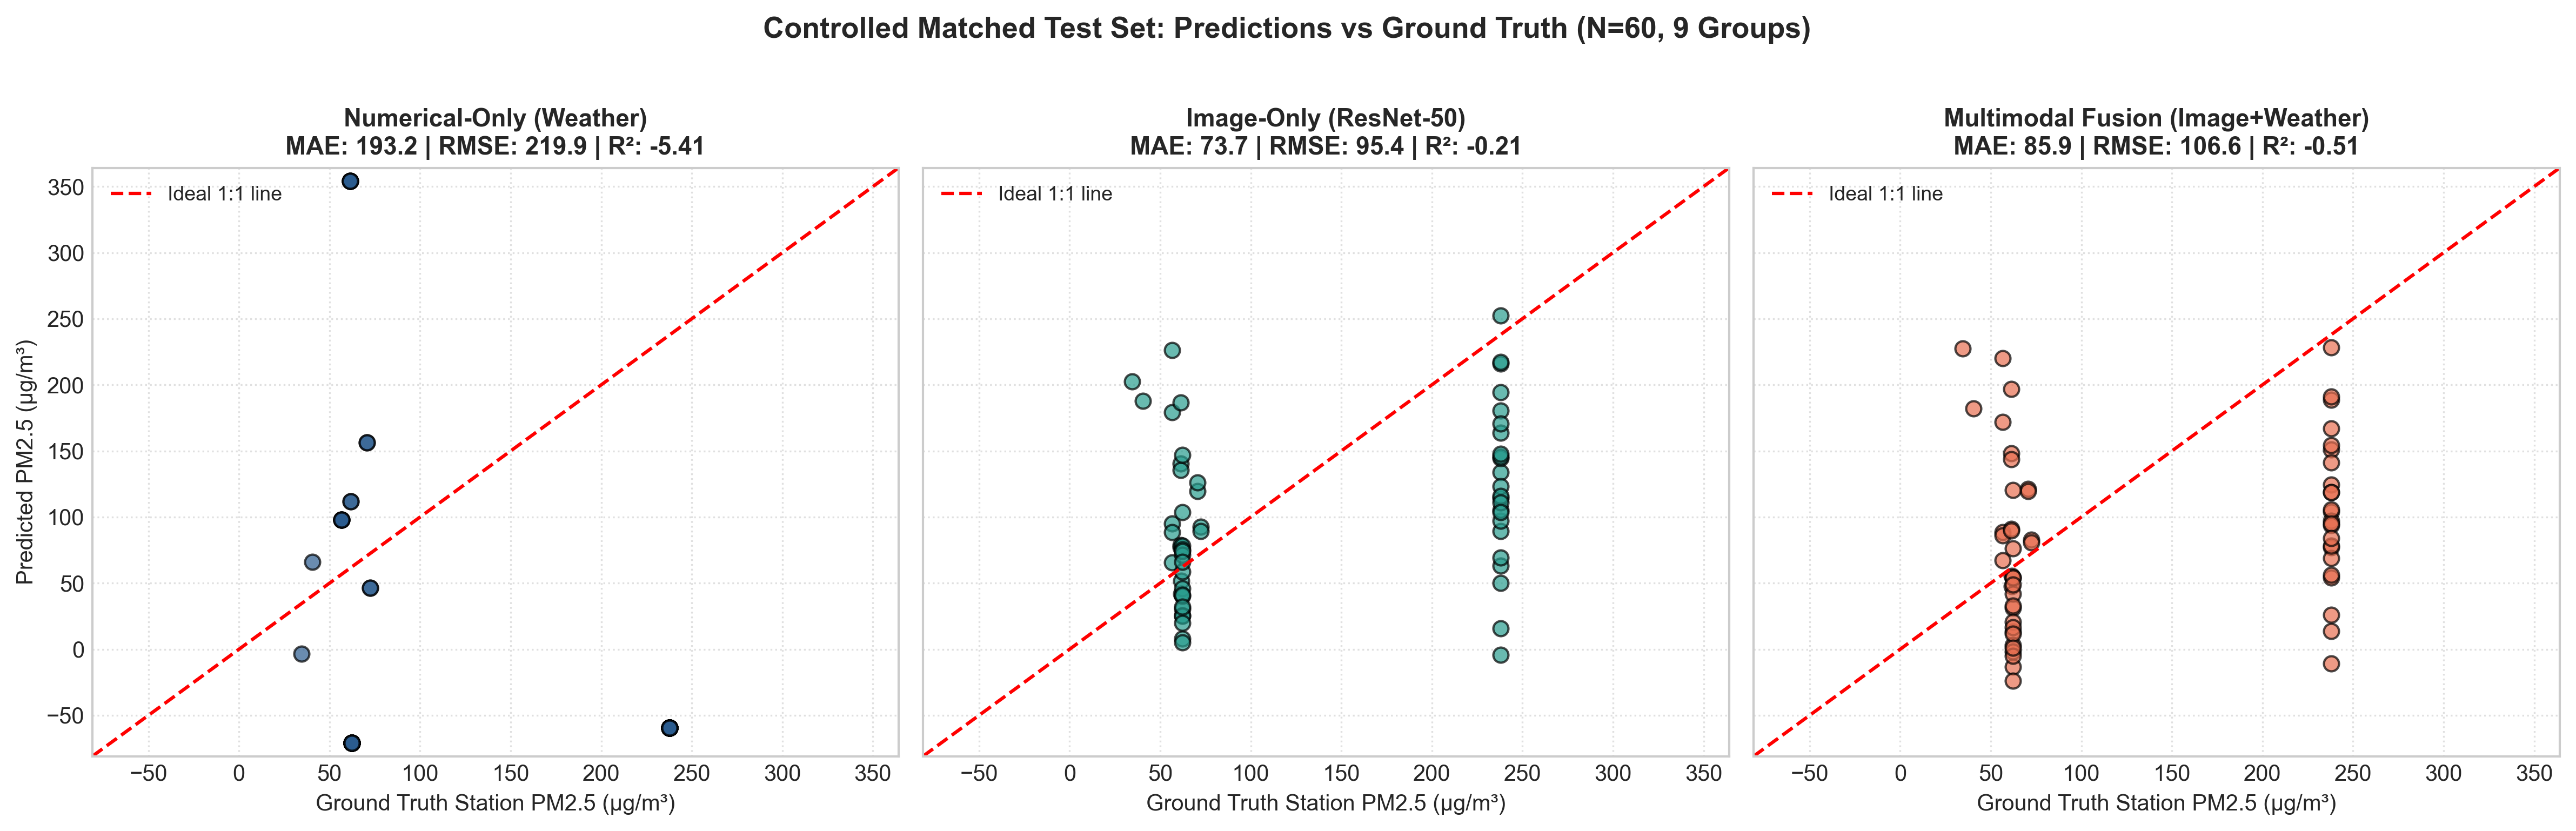
\includegraphics[width=\textwidth]{matched_predictions_vs_ground_truth.png}
\caption{Controlled matched test set evaluations ($N=60$ samples across 9 held-out station-date groups): Predictions versus ground-truth station $\text{PM}_{2.5}$ for (a) Numerical Weather-Only; (b) ResNet-50 Image-Only; and (c) Multimodal Early Fusion.}
\label{fig:predictions}
\end{figure*}

\section{Results and Discussion}

\subsection{Comprehensive Model Comparison}
Table~\ref{tab:results} summarizes the performance across all evaluated model paradigms. The results must not be conflated across rows: the LSTM predicts operational hourly concentrations over 404,431 sequences, the ResNet-50 evaluates image-level PM estimation on 79 unseen groups, and the matched models evaluate daily station ground truth on 60 matched instances.

\begin{table*}[t]
\caption{Comprehensive Performance Benchmark Across All Evaluated Air Quality Paradigms}
\label{tab:results}
\centering
\begin{tabular}{lllcrrrr}
\toprule
\textbf{Paradigm / Context} & \textbf{Model} & \textbf{Modality} & \textbf{Target} & \textbf{Test $N$} & \textbf{MAE} & \textbf{RMSE} & \textbf{$R^2$} \\
\midrule
\multirow{4}{*}{\shortstack[l]{\textbf{Operational Forecasting}\\(Continuous 1-hour ahead)}} 
& 2-Layer LSTM Forecaster & Numerical (AQ + Weather) & $\text{PM}_{2.5}$ & 404,431 & \textbf{10.5719} & \textbf{18.5789} & \textbf{0.9492} \\
& 2-Layer LSTM Forecaster & Numerical (AQ + Weather) & $\text{PM}_{10}$  & 404,431 & \textbf{18.8643} & \textbf{32.2027} & \textbf{0.9301} \\
& Persistence Benchmark   & Numerical (Lagged $\text{PM}_t$) & $\text{PM}_{2.5}$ & 404,431 & 10.6783 & 19.8072 & 0.9423 \\
& Persistence Benchmark   & Numerical (Lagged $\text{PM}_t$) & $\text{PM}_{10}$  & 404,431 & 19.7384 & 36.2374 & 0.9115 \\
\midrule
\textbf{Environmental Vision} & ResNet-50 Transfer & Image-only (PM25Vision) & $\text{PM}_{2.5}$ & 79 & 66.2148 & 80.6779 & 0.1524 \\
\midrule
\multirow{6}{*}{\shortstack[l]{\textbf{Exploratory Matched Cohort}\\(Station Daily Ground Truth,\\Held-out 9 Test Groups)}} 
& Numerical Ridge & Daily ERA5-Land Weather & $\text{PM}_{2.5}$ & 60 & 193.1787 & 219.8654 & -5.4129 \\
& Image Ridge & ResNet-50 Features & $\text{PM}_{2.5}$ & 60 & \textbf{73.6699} & \textbf{95.3836} & \textbf{-0.2070} \\
& Multimodal Early Fusion & Image + Weather Features & $\text{PM}_{2.5}$ & 60 & 85.8619 & 106.5622 & -0.5064 \\
\cmidrule{2-8}
& Numerical Ridge & Daily ERA5-Land Weather & $\text{PM}_{10}$  & 60 & 297.1218 & 349.2314 & -3.2755 \\
& Image Ridge & ResNet-50 Features & $\text{PM}_{10}$  & 60 & \textbf{137.6515} & \textbf{172.1311} & \textbf{-0.0387} \\
& Multimodal Early Fusion & Image + Weather Features & $\text{PM}_{10}$  & 60 & 150.4686 & 186.1649 & -0.2150 \\
\bottomrule
\end{tabular}
\end{table*}

\subsection{Numerical Forecasting Performance}
The 2-layer LSTM forecaster achieved a test MAE of 10.5719 $\mu\text{g/m}^3$ and $R^2$ of 0.9492 for $\text{PM}_{2.5}$, and an MAE of 18.8643 $\mu\text{g/m}^3$ ($R^2 = 0.9301$) for $\text{PM}_{10}$ on 404,431 held-out test sequences. As illustrated in Fig.~\ref{fig:regression_metrics}, the LSTM model consistently outperformed the 1-hour persistence baseline ($\text{PM}_{2.5}$ MAE: 10.6783 $\mu\text{g/m}^3$, RMSE: 19.8072 $\mu\text{g/m}^3$, $R^2 = 0.9423$; $\text{PM}_{10}$ MAE: 19.7384 $\mu\text{g/m}^3$, RMSE: 36.2374 $\mu\text{g/m}^3$, $R^2 = 0.9115$), yielding an RMSE reduction of 6.2\% for $\text{PM}_{2.5}$ and 11.1\% for $\text{PM}_{10}$. Physical concentration errors are reported in $\mu\text{g/m}^3$ on panel (a), while dimensionless variance explained ($R^2$) is reported separately on panel (b) to prevent scale conflation.

\begin{figure}[t]
\centering
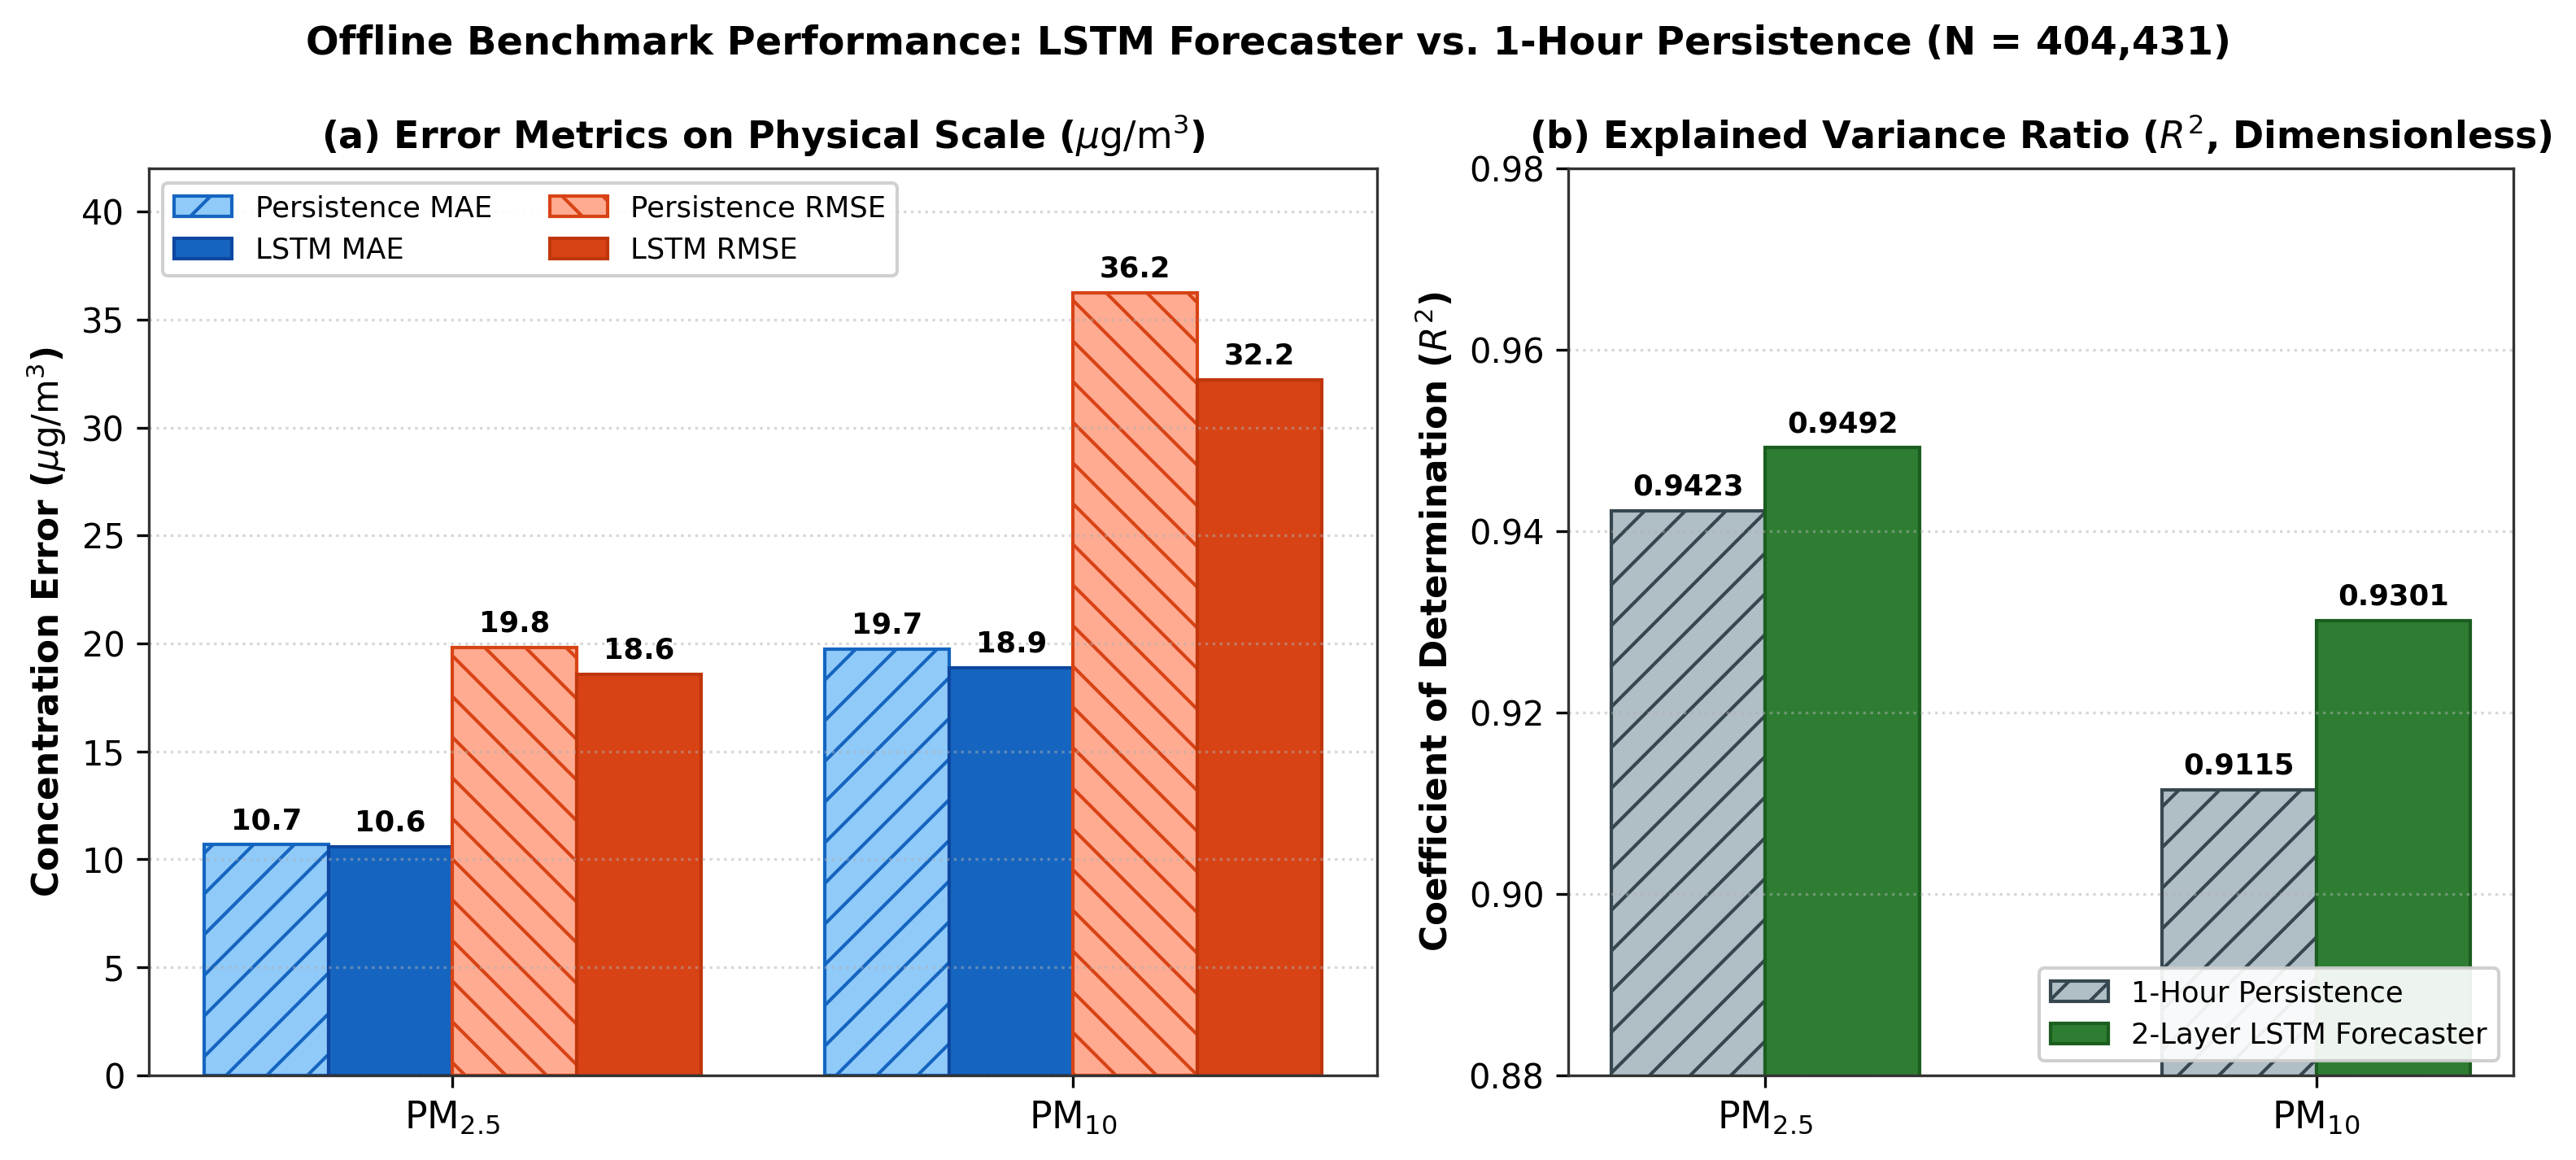
\includegraphics[width=\columnwidth]{figures/regression_metrics.png}
\caption{Offline benchmark comparison between the 2-layer LSTM forecaster and 1-hour persistence baseline across 404,431 held-out test sequences: (a) Error metrics on physical scale (MAE and RMSE in $\mu\text{g/m}^3$); (b) Explained variance ratio ($R^2$, dimensionless).}
\label{fig:regression_metrics}
\end{figure}

\begin{figure*}[t]
\centering
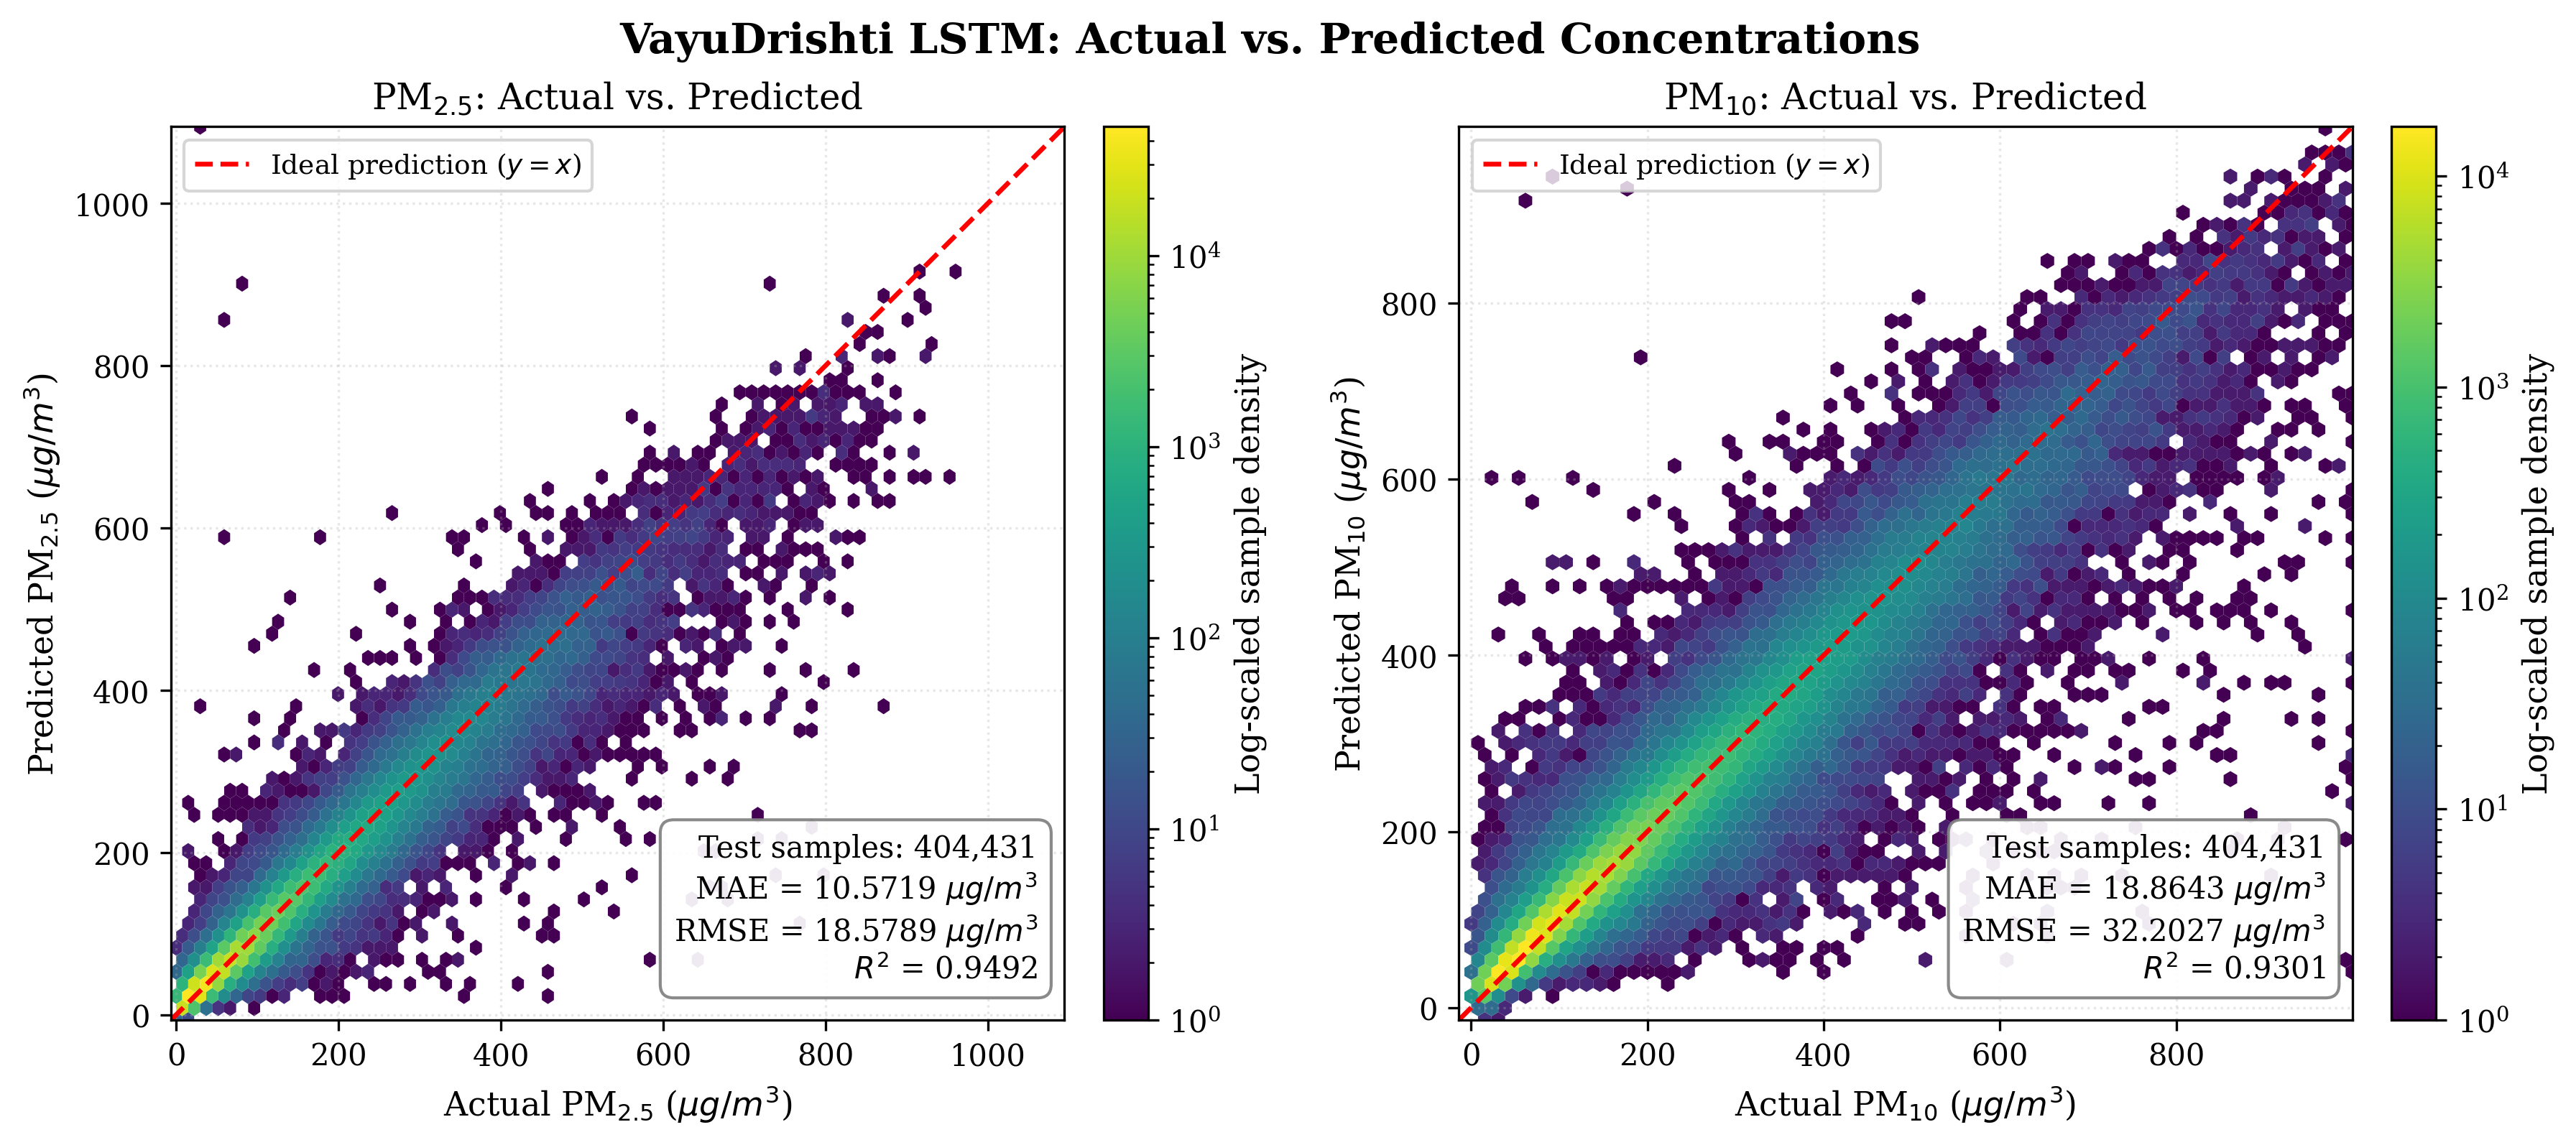
\includegraphics[width=\textwidth]{figures/actual_vs_predicted.png}
\caption{Offline test set continuous concentration evaluation: Ground-truth observed versus LSTM next-hour predicted concentrations across 404,431 held-out sequences for (a) $\text{PM}_{2.5}$ and (b) $\text{PM}_{10}$. The red dashed line denotes ideal 1:1 concordance ($y = x$). Density shading visualizes point distribution over a reproducible random subsample ($n = 12,000$, seed=42) to prevent visual saturation while reporting full-test metrics in the inset.}
\label{fig:actual_vs_predicted}
\end{figure*}

\begin{figure*}[t]
\centering
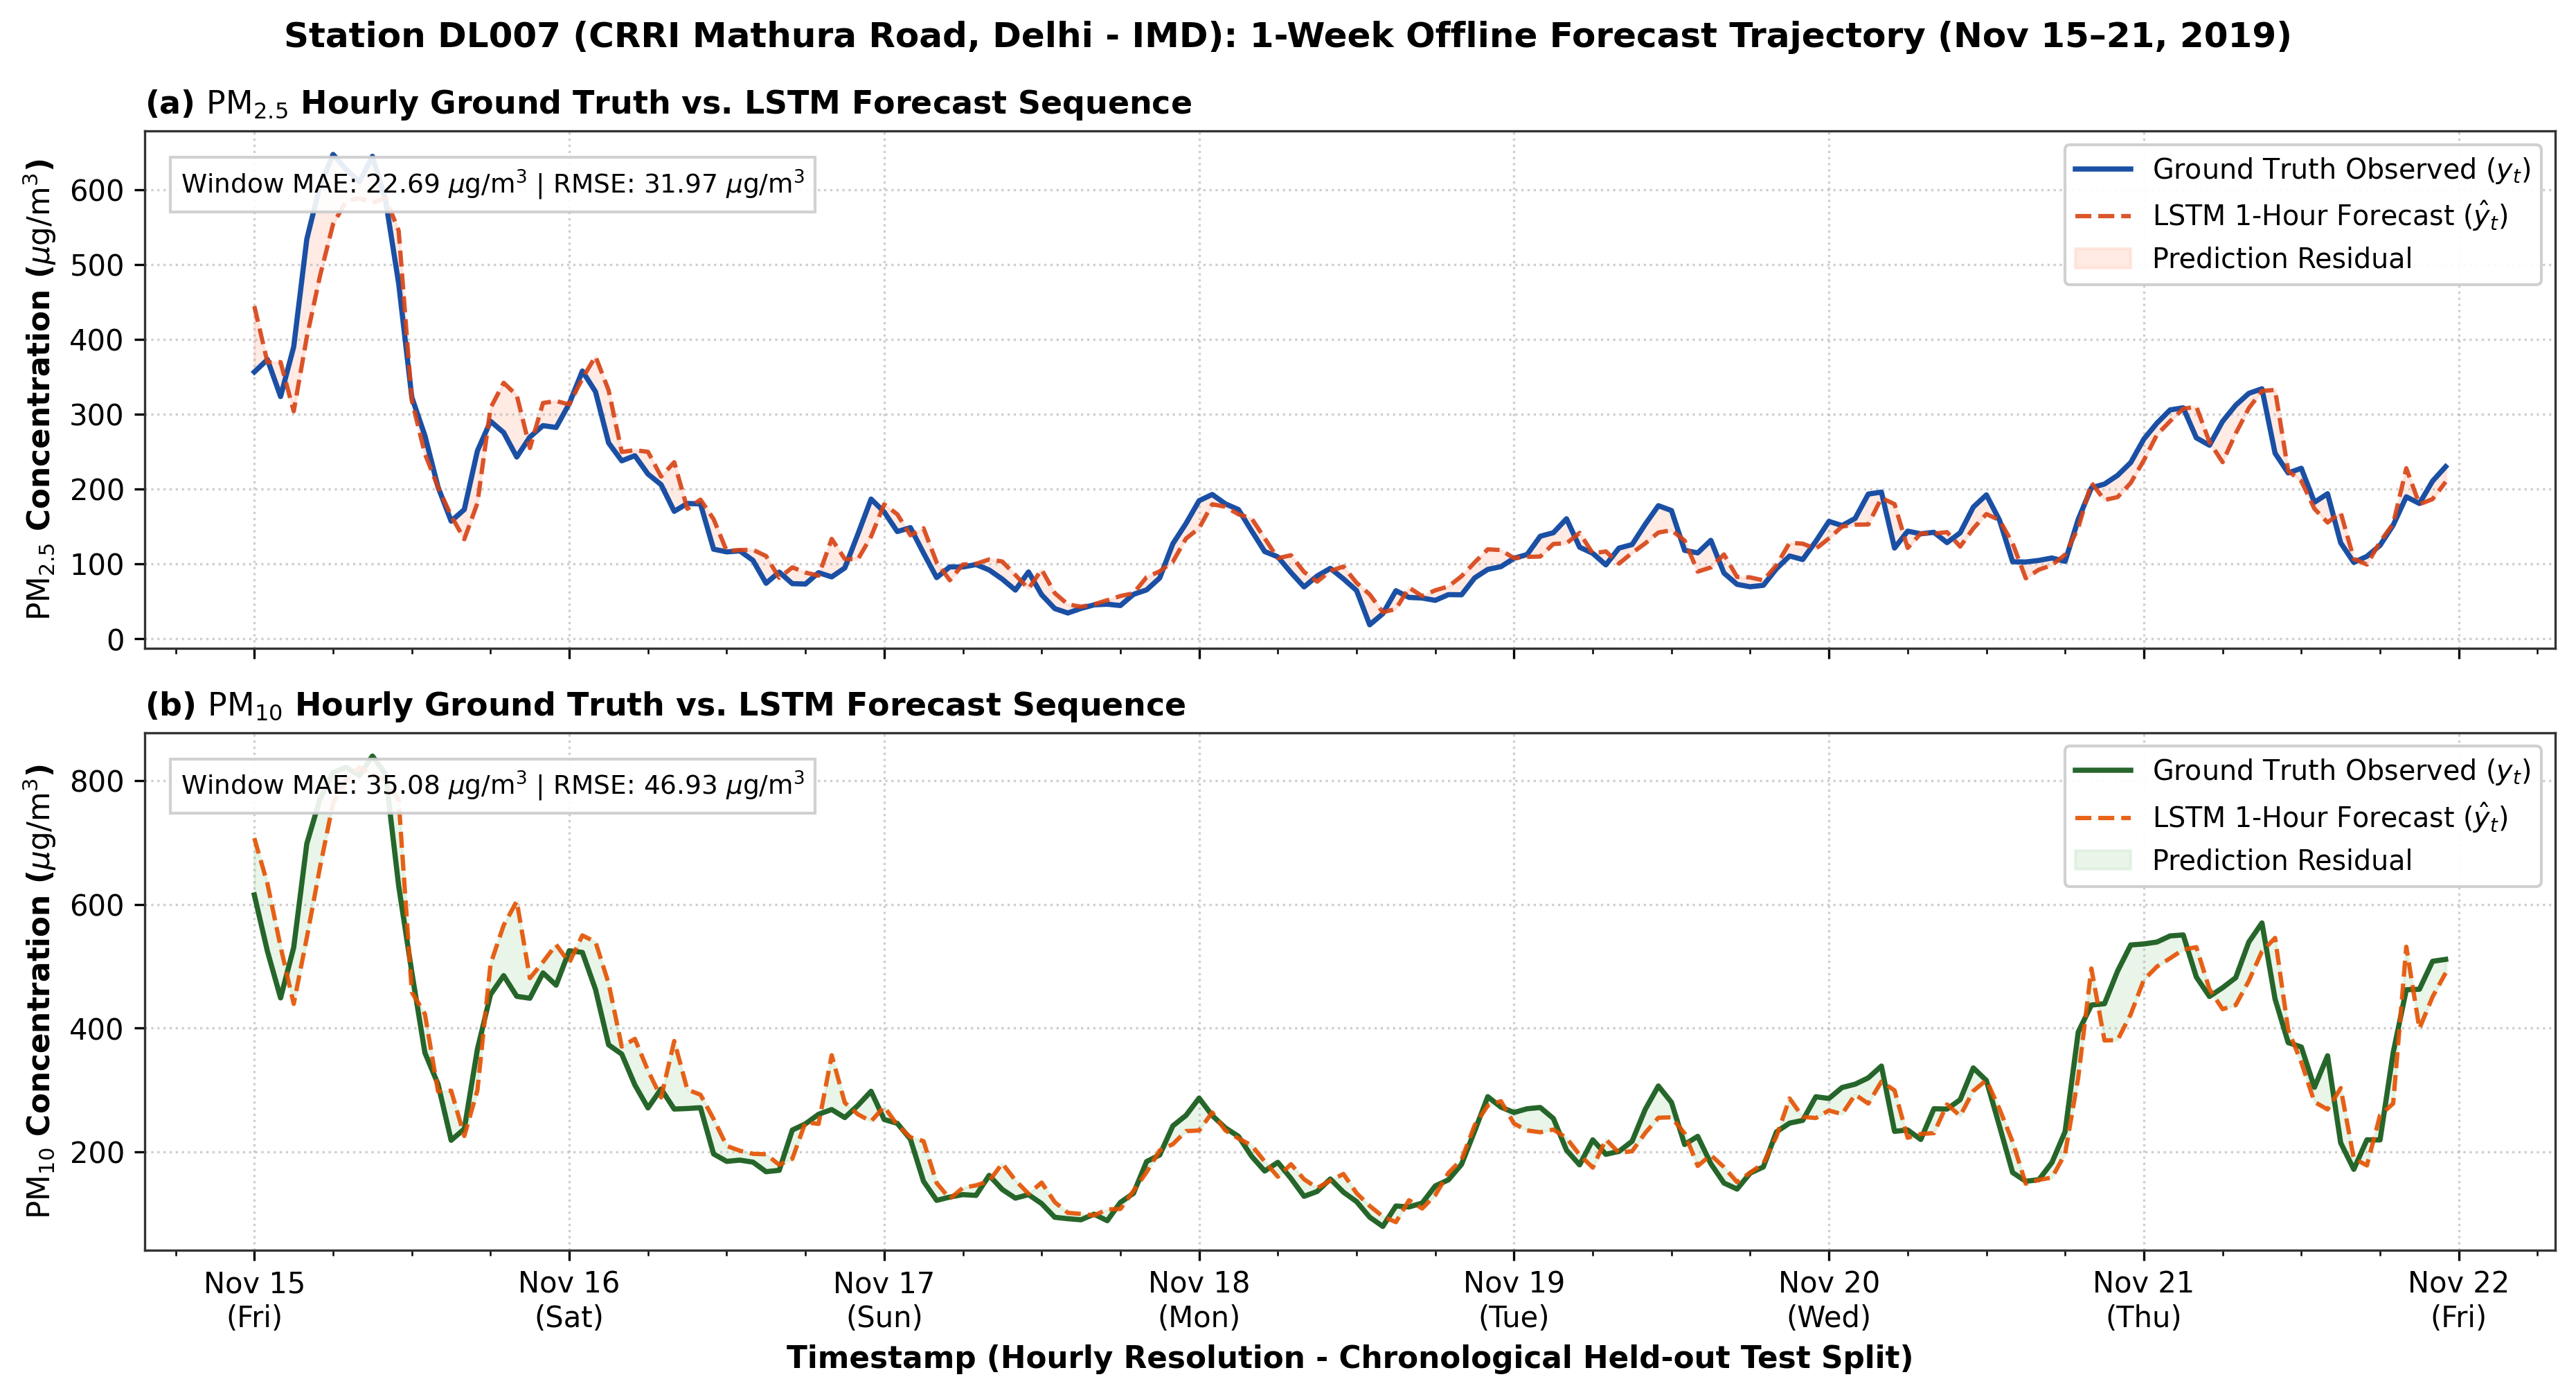
\includegraphics[width=\textwidth]{figures/prediction_timeseries.png}
\caption{Continuous 168-hour offline forecasting trajectory at monitoring station DL007 (CRRI Mathura Road, Delhi - IMD; Lat: 28.56$^\circ$N, Lon: 77.20$^\circ$E) over November 15--21, 2019: (a) $\text{PM}_{2.5}$ hourly ground truth versus LSTM next-hour predictions; (b) $\text{PM}_{10}$ hourly ground truth versus LSTM next-hour predictions, with shaded prediction residuals.}
\label{fig:prediction_timeseries}
\end{figure*}

Fig.~\ref{fig:actual_vs_predicted} provides a scatter and density visualization of observed versus predicted concentrations across the full spectrum of air quality conditions. The model maintains tight clustering around the $y=x$ concordance line across both moderate and high concentration ranges. To examine temporal tracking fidelity under real urban conditions, Fig.~\ref{fig:prediction_timeseries} plots a continuous 1-week (168-hour) test trajectory for station DL007 in Delhi. The LSTM forecaster accurately captures diurnal pollution crests and troughs, maintaining low residual errors even during rapid concentration transitions.

\subsubsection{Exploratory Concentration-Category Evaluation}
To assess operational interpretability for public health advisory, continuous concentration predictions and observations were mapped into six discrete categories using the concentration breakpoints defined in the Indian Central Pollution Control Board (CPCB) National Air Quality Index (NAQI) guidelines (Good: 0--30 $\mu\text{g/m}^3$ $\text{PM}_{2.5}$, 0--50 $\mu\text{g/m}^3$ $\text{PM}_{10}$; Satisfactory: 30--60 $\mu\text{g/m}^3$ $\text{PM}_{2.5}$, 50--100 $\mu\text{g/m}^3$ $\text{PM}_{10}$; Moderate: 60--90 $\mu\text{g/m}^3$ $\text{PM}_{2.5}$, 100--250 $\mu\text{g/m}^3$ $\text{PM}_{10}$; Poor: 90--120 $\mu\text{g/m}^3$ $\text{PM}_{2.5}$, 250--350 $\mu\text{g/m}^3$ $\text{PM}_{10}$; Very Poor: 120--250 $\mu\text{g/m}^3$ $\text{PM}_{2.5}$, 350--430 $\mu\text{g/m}^3$ $\text{PM}_{10}$; Severe: $>250$ $\mu\text{g/m}^3$ $\text{PM}_{2.5}$, $>430$ $\mu\text{g/m}^3$ $\text{PM}_{10}$).

On the full held-out test set ($N = 404,431$ sequences; 0 excluded):
\begin{itemize}
    \item \textbf{Exact Category Accuracy}: \textbf{77.04\%} for $\text{PM}_{2.5}$ and \textbf{80.88\%} for $\text{PM}_{10}$.
    \item \textbf{Macro-Averaged F1-Score}: \textbf{0.7657} for $\text{PM}_{2.5}$ and \textbf{0.7504} for $\text{PM}_{10}$.
    \item \textbf{Weighted-Averaged F1-Score}: \textbf{0.7731} for $\text{PM}_{2.5}$ and \textbf{0.8075} for $\text{PM}_{10}$.
    \item \textbf{Adjacent-Category Accuracy ($\pm 1$ bin tolerance)}: \textbf{99.35\%} for $\text{PM}_{2.5}$ and \textbf{99.48\%} for $\text{PM}_{10}$.
\end{itemize}

\begin{figure}[t]
\centering
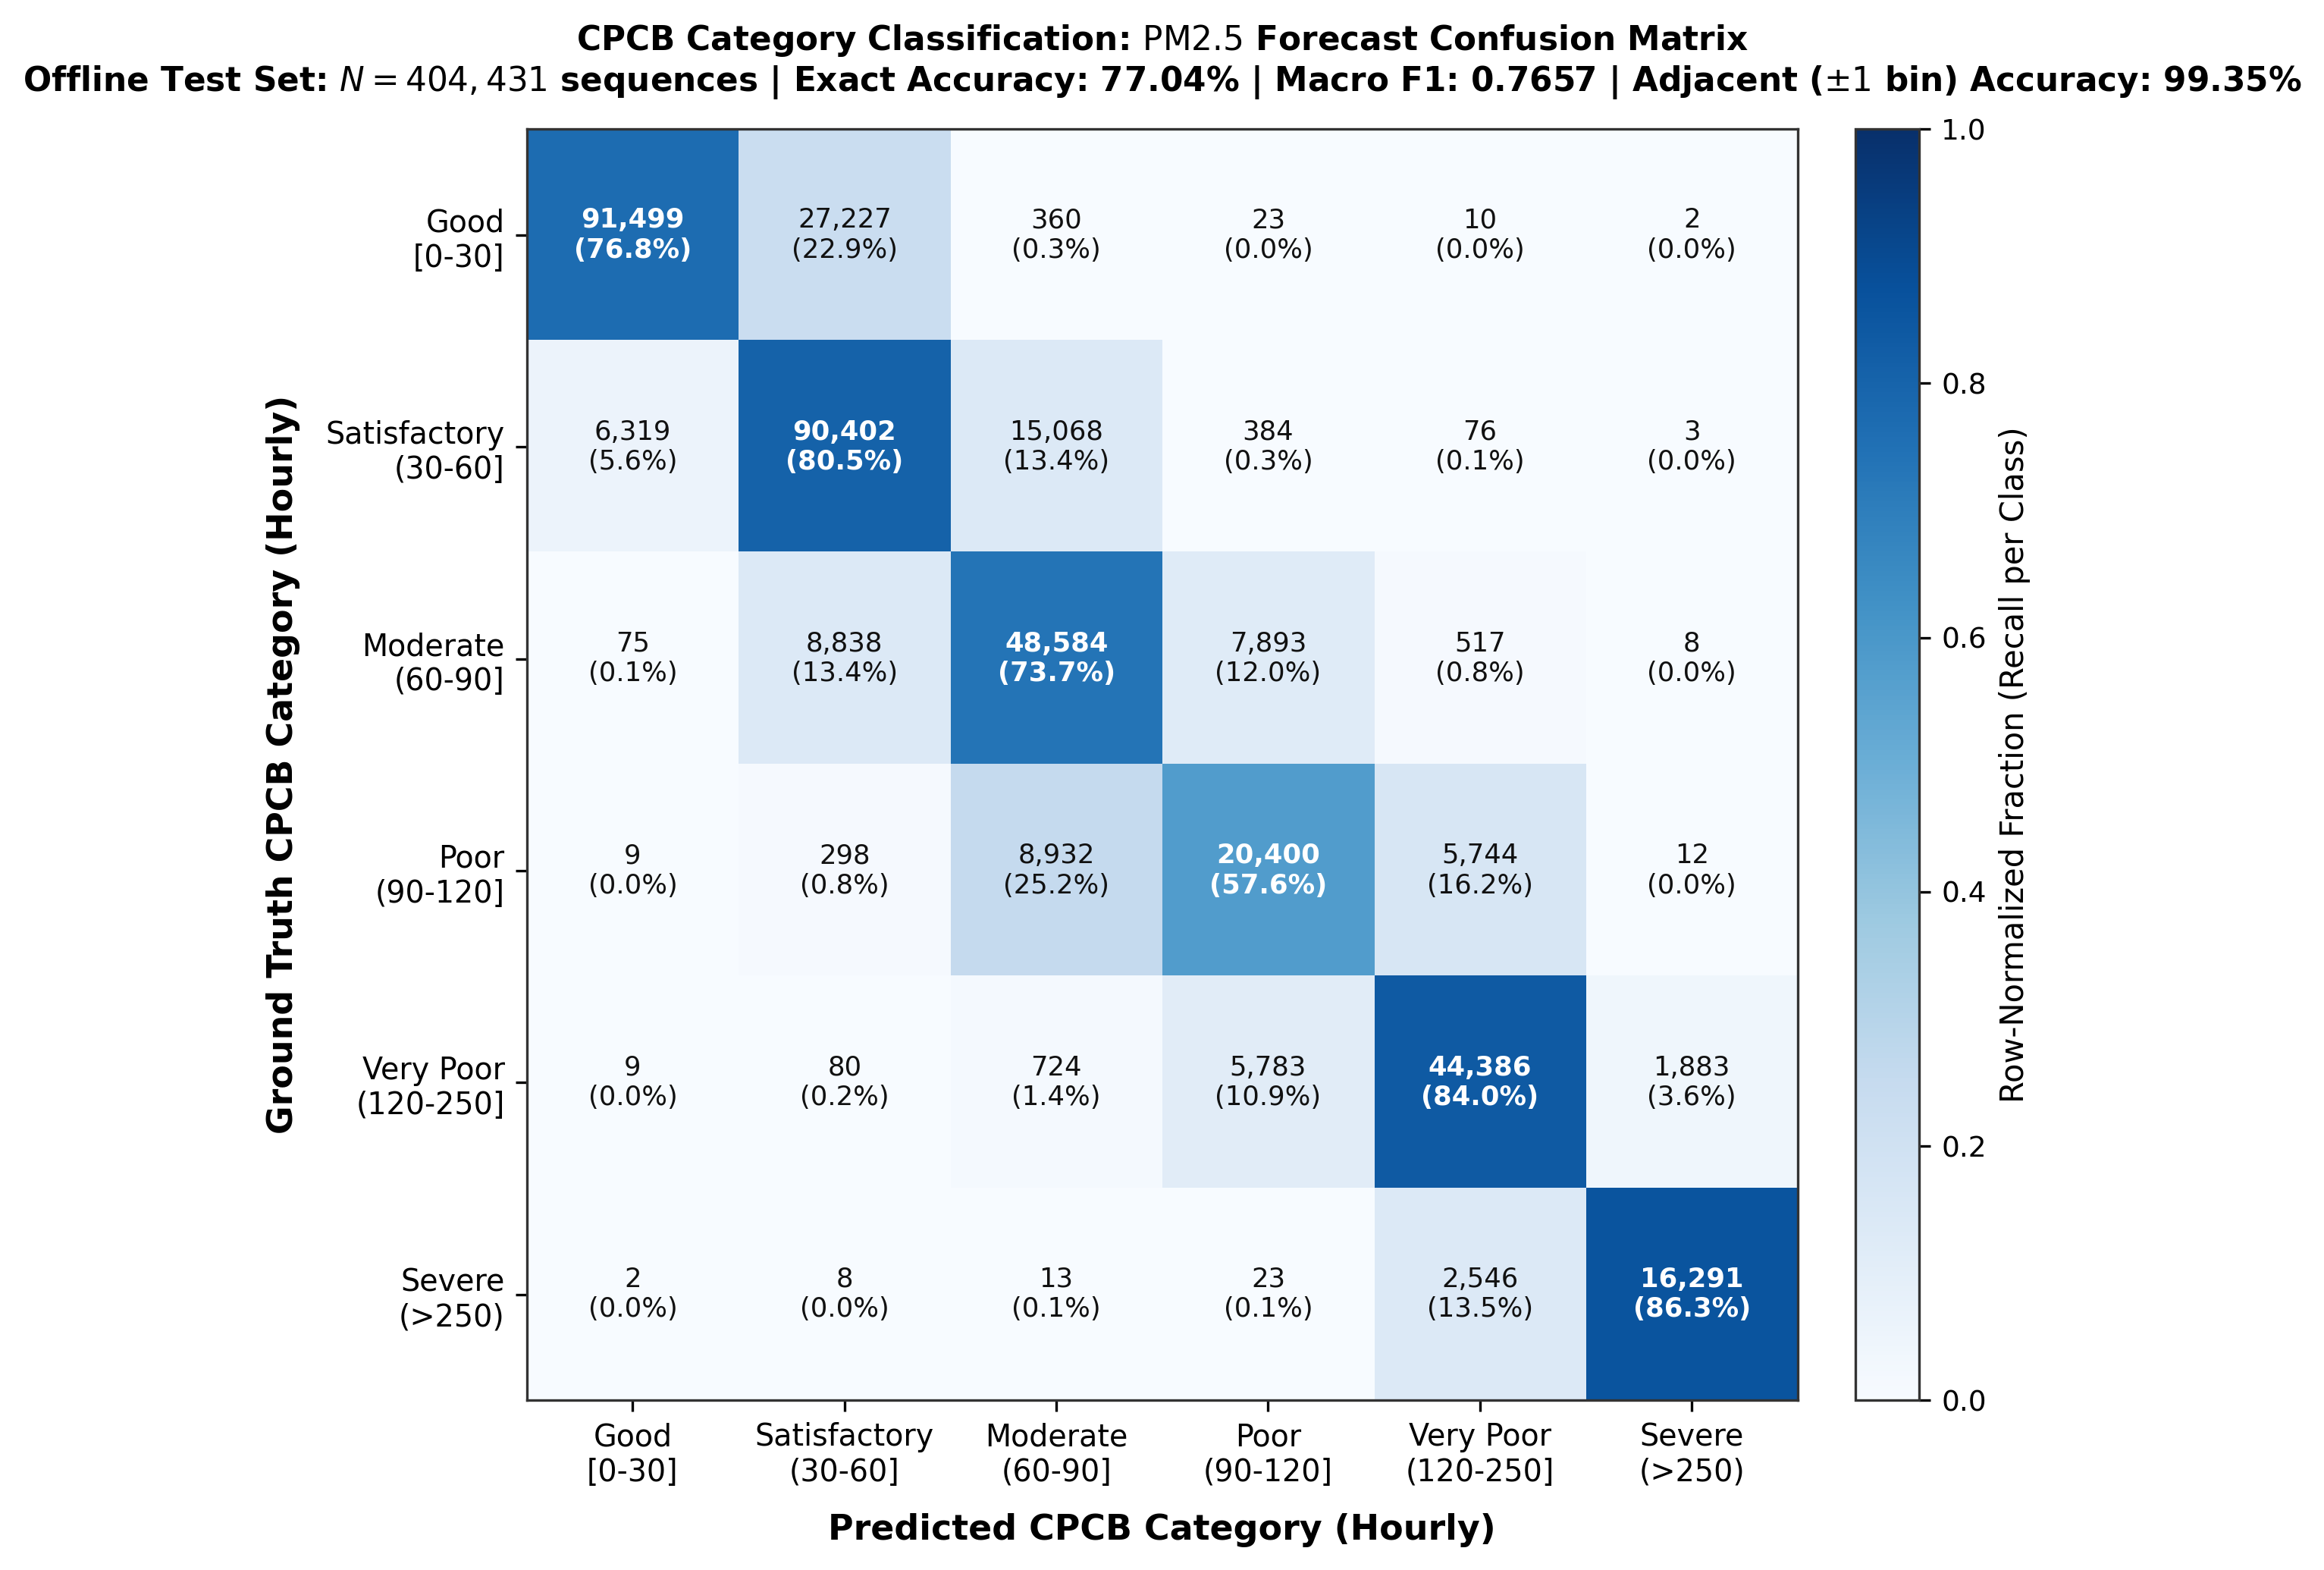
\includegraphics[width=\columnwidth]{figures/confusion_matrix_pm25.png}
\caption{CPCB category confusion matrix for $\text{PM}_{2.5}$ hourly predictions evaluated on 404,431 offline test sequences. Each cell displays absolute sequence counts and row-normalized recall percentages.}
\label{fig:cm_pm25}
\end{figure}

\begin{figure}[t]
\centering
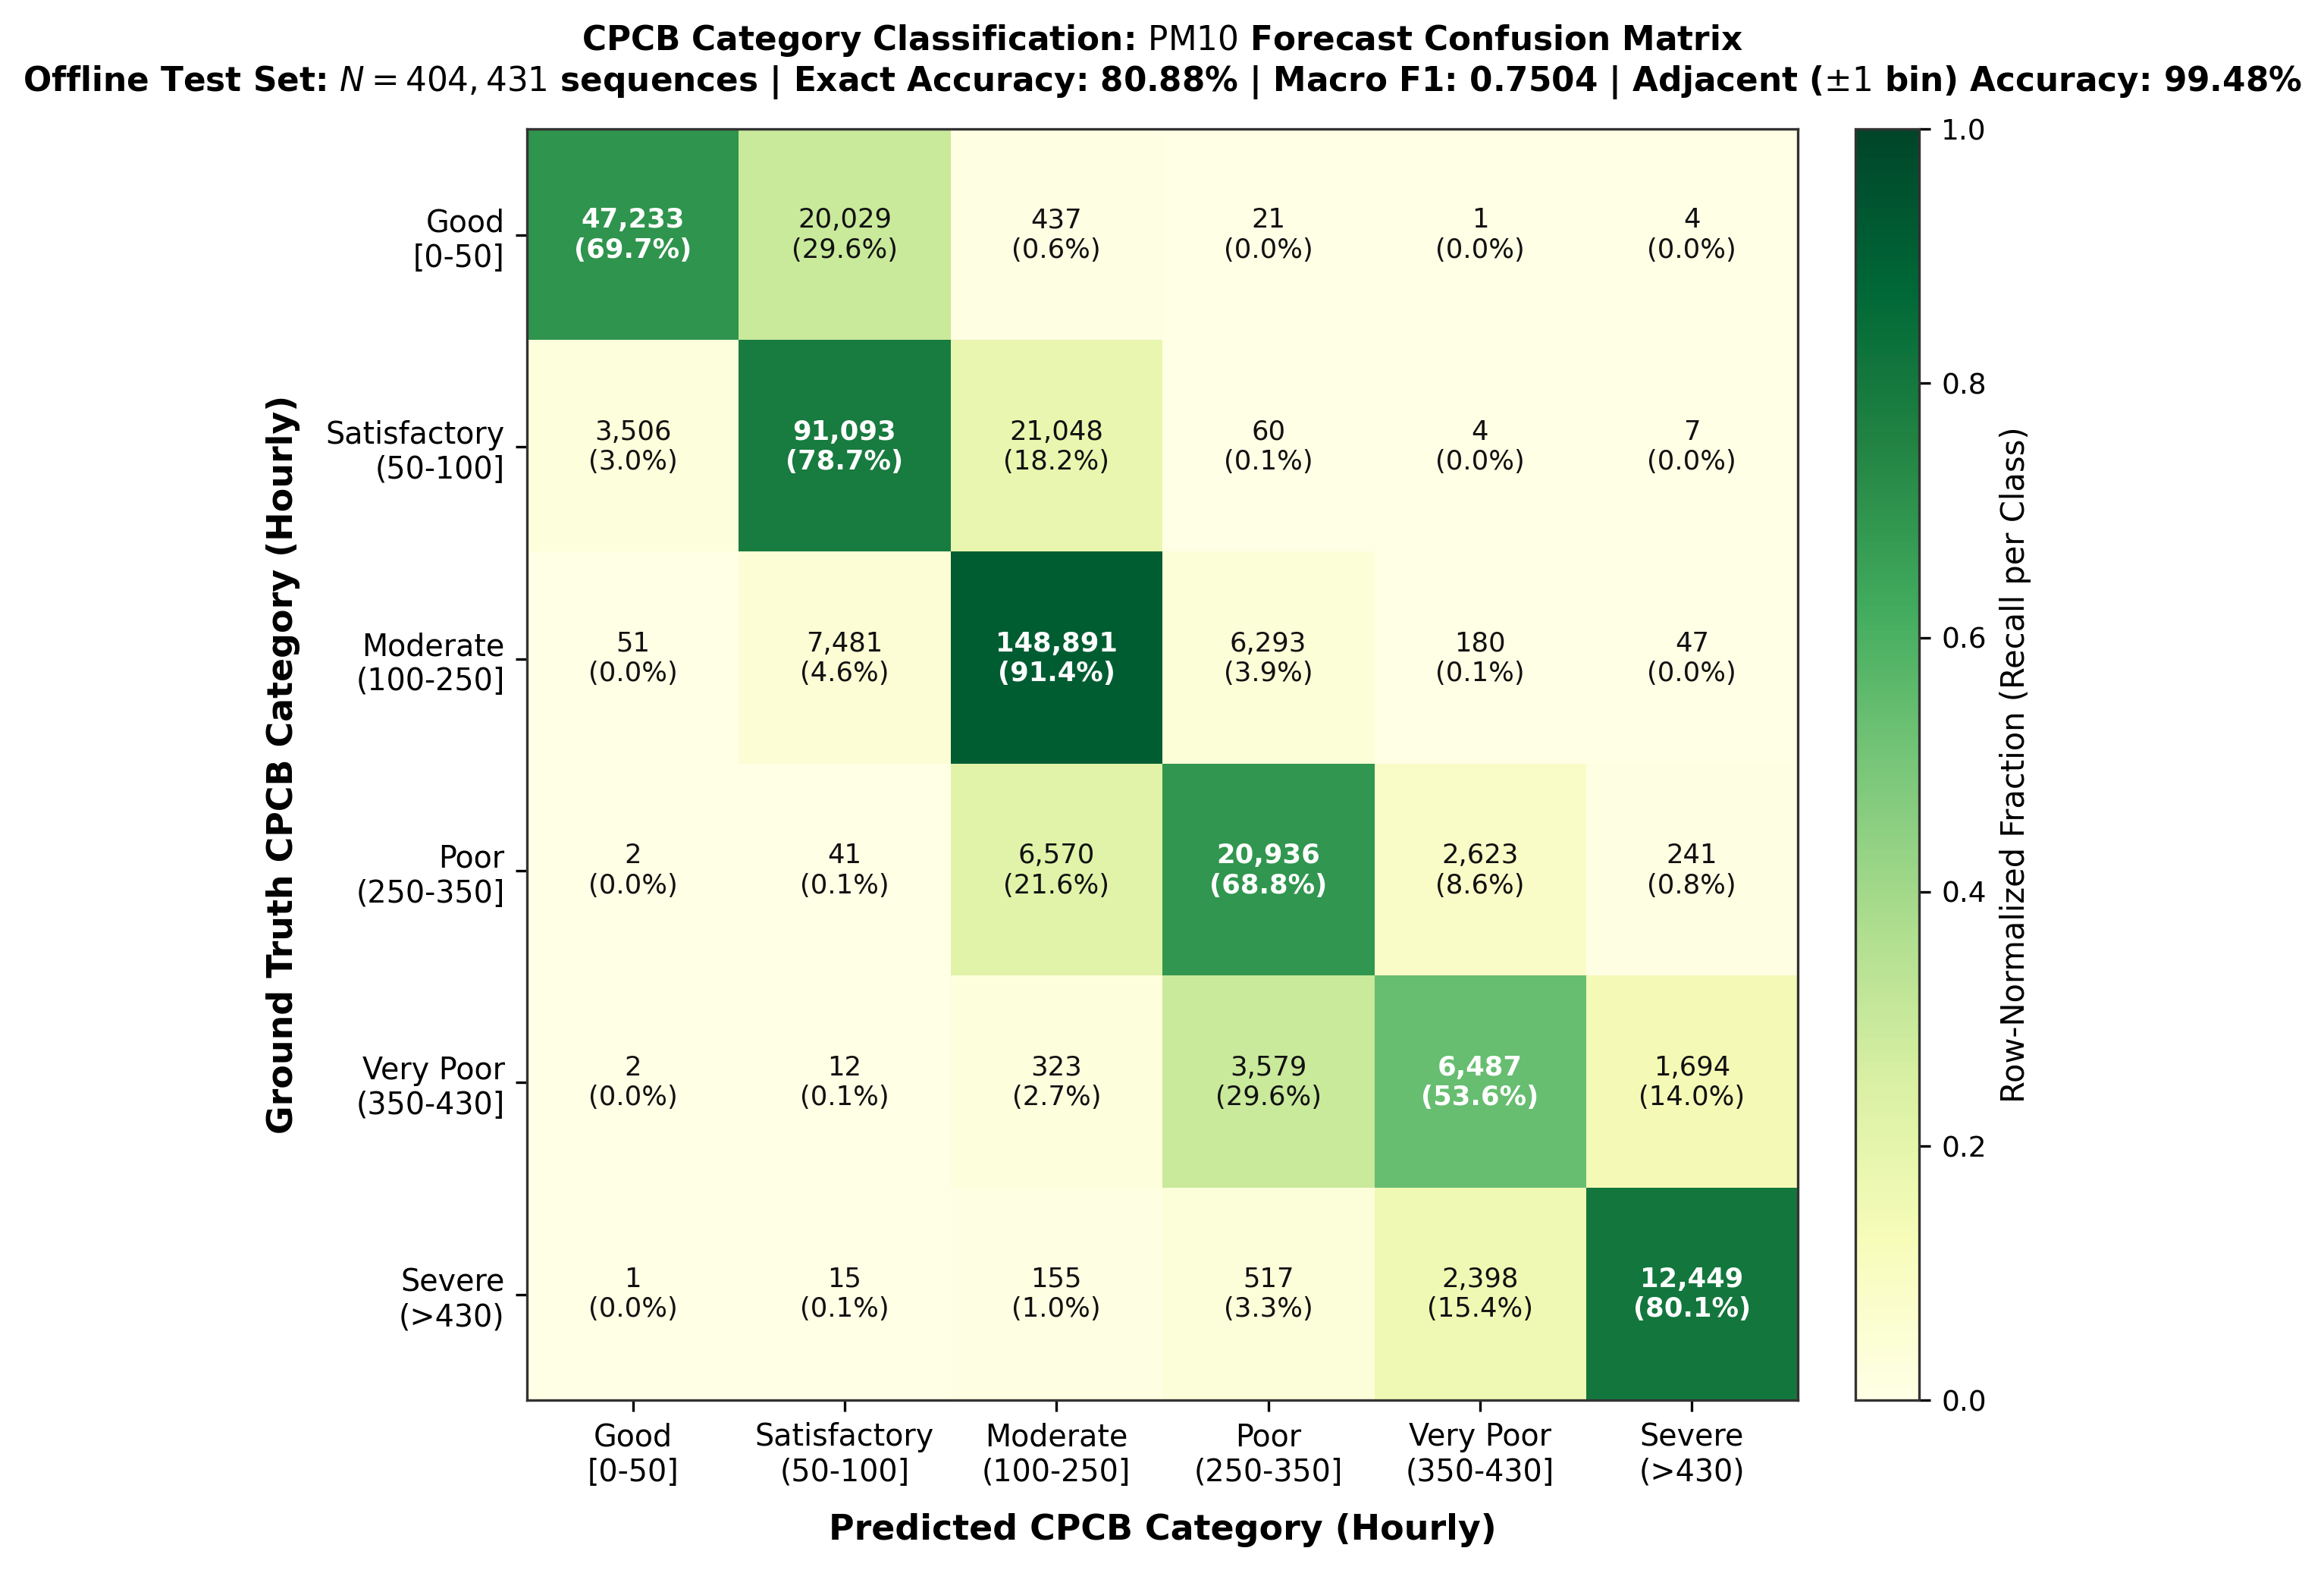
\includegraphics[width=\columnwidth]{figures/confusion_matrix_pm10.png}
\caption{CPCB category confusion matrix for $\text{PM}_{10}$ hourly predictions evaluated on 404,431 offline test sequences. Each cell displays absolute sequence counts and row-normalized recall percentages.}
\label{fig:cm_pm10}
\end{figure}

The resulting confusion matrices are presented in Fig.~\ref{fig:cm_pm25} ($\text{PM}_{2.5}$) and Fig.~\ref{fig:cm_pm10} ($\text{PM}_{10}$). For both pollutants, the mass of the distribution is concentrated strictly along the diagonal and immediate adjacent off-diagonals, corroborating the $>99.3\%$ adjacent-category accuracy.

\noindent\textbf{Methodological Limitations and Boundary Context}:
\begin{enumerate}
    \item \textit{Averaging Period Discrepancy}: Official CPCB NAQI breakpoints are calibrated for 24-hour truncated averages. Because the operational LSTM operates on 1-hour ahead sequence forecasting, applying these thresholds to hourly values serves as an exploratory operational benchmark rather than a statutory regulatory compliance determination.
    \item \textit{Sub-Index vs. Composite NAQI}: Official Indian AQI is a multi-pollutant composite requiring at least three active pollutants, including particulate matter. These categorical results assess single-pollutant concentration bin classification and must not be construed as official multi-pollutant composite AQI accuracy.
    \item \textit{Boundary Sensitivity}: Misclassifications are overwhelmingly concentrated at boundary thresholds (e.g., 29.5 vs 30.5 $\mu\text{g/m}^3$ across the Good/Satisfactory frontier), with multi-tier errors occurring in under 0.65\% of test observations.
\end{enumerate}

\subsection{Image-Only Baseline Performance}
The ResNet-50 baseline yielded an MAE of 66.2148 $\mu\text{g/m}^3$ ($R^2 = 0.1524$) on the held-out test split of 79 images across 18 unseen station-date groups. Given that ambient particulate concentrations in urban India span from $<20$ to $>450\ \mu\text{g/m}^3$, an $R^2$ of 0.15 indicates that deep optical features capture general haze levels, though accuracy remains coarse compared to sensor telemetry.

\subsection{Exploratory Fusion Findings: A Negative Result}
The controlled matched experiment provides a critical empirical insight:
\begin{enumerate}
    \item \textbf{Weather-Only Failure}: The Numerical Weather-Only model collapsed out-of-sample ($R^2 = -5.4129$), indicating that static daily meteorological averages without historical sequence context or station identity cannot infer absolute particulate levels across unseen cities.
    \item \textbf{Image Features Outperform Weather}: The Image-Only model achieved an MAE of 73.6699 $\mu\text{g/m}^3$ ($R^2 = -0.2070$), capturing localized visual haze significantly better than weather alone.
    \item \textbf{Multimodal Fusion Degrades Performance}: Multimodal Early Fusion achieved an MAE of 85.8619 $\mu\text{g/m}^3$ ($R^2 = -0.5064$), performing \textbf{12.19 $\mu\text{g/m}^3$ worse} than Image-Only. In Fig.~\ref{fig:predictions}, both Image-Only and Multimodal models display conservative shrinkage toward the training mean, but the multimodal model incurs higher variance from over-parameterized feature concatenation on only 27 training groups.
\end{enumerate}

\begin{figure}[t]
\centering
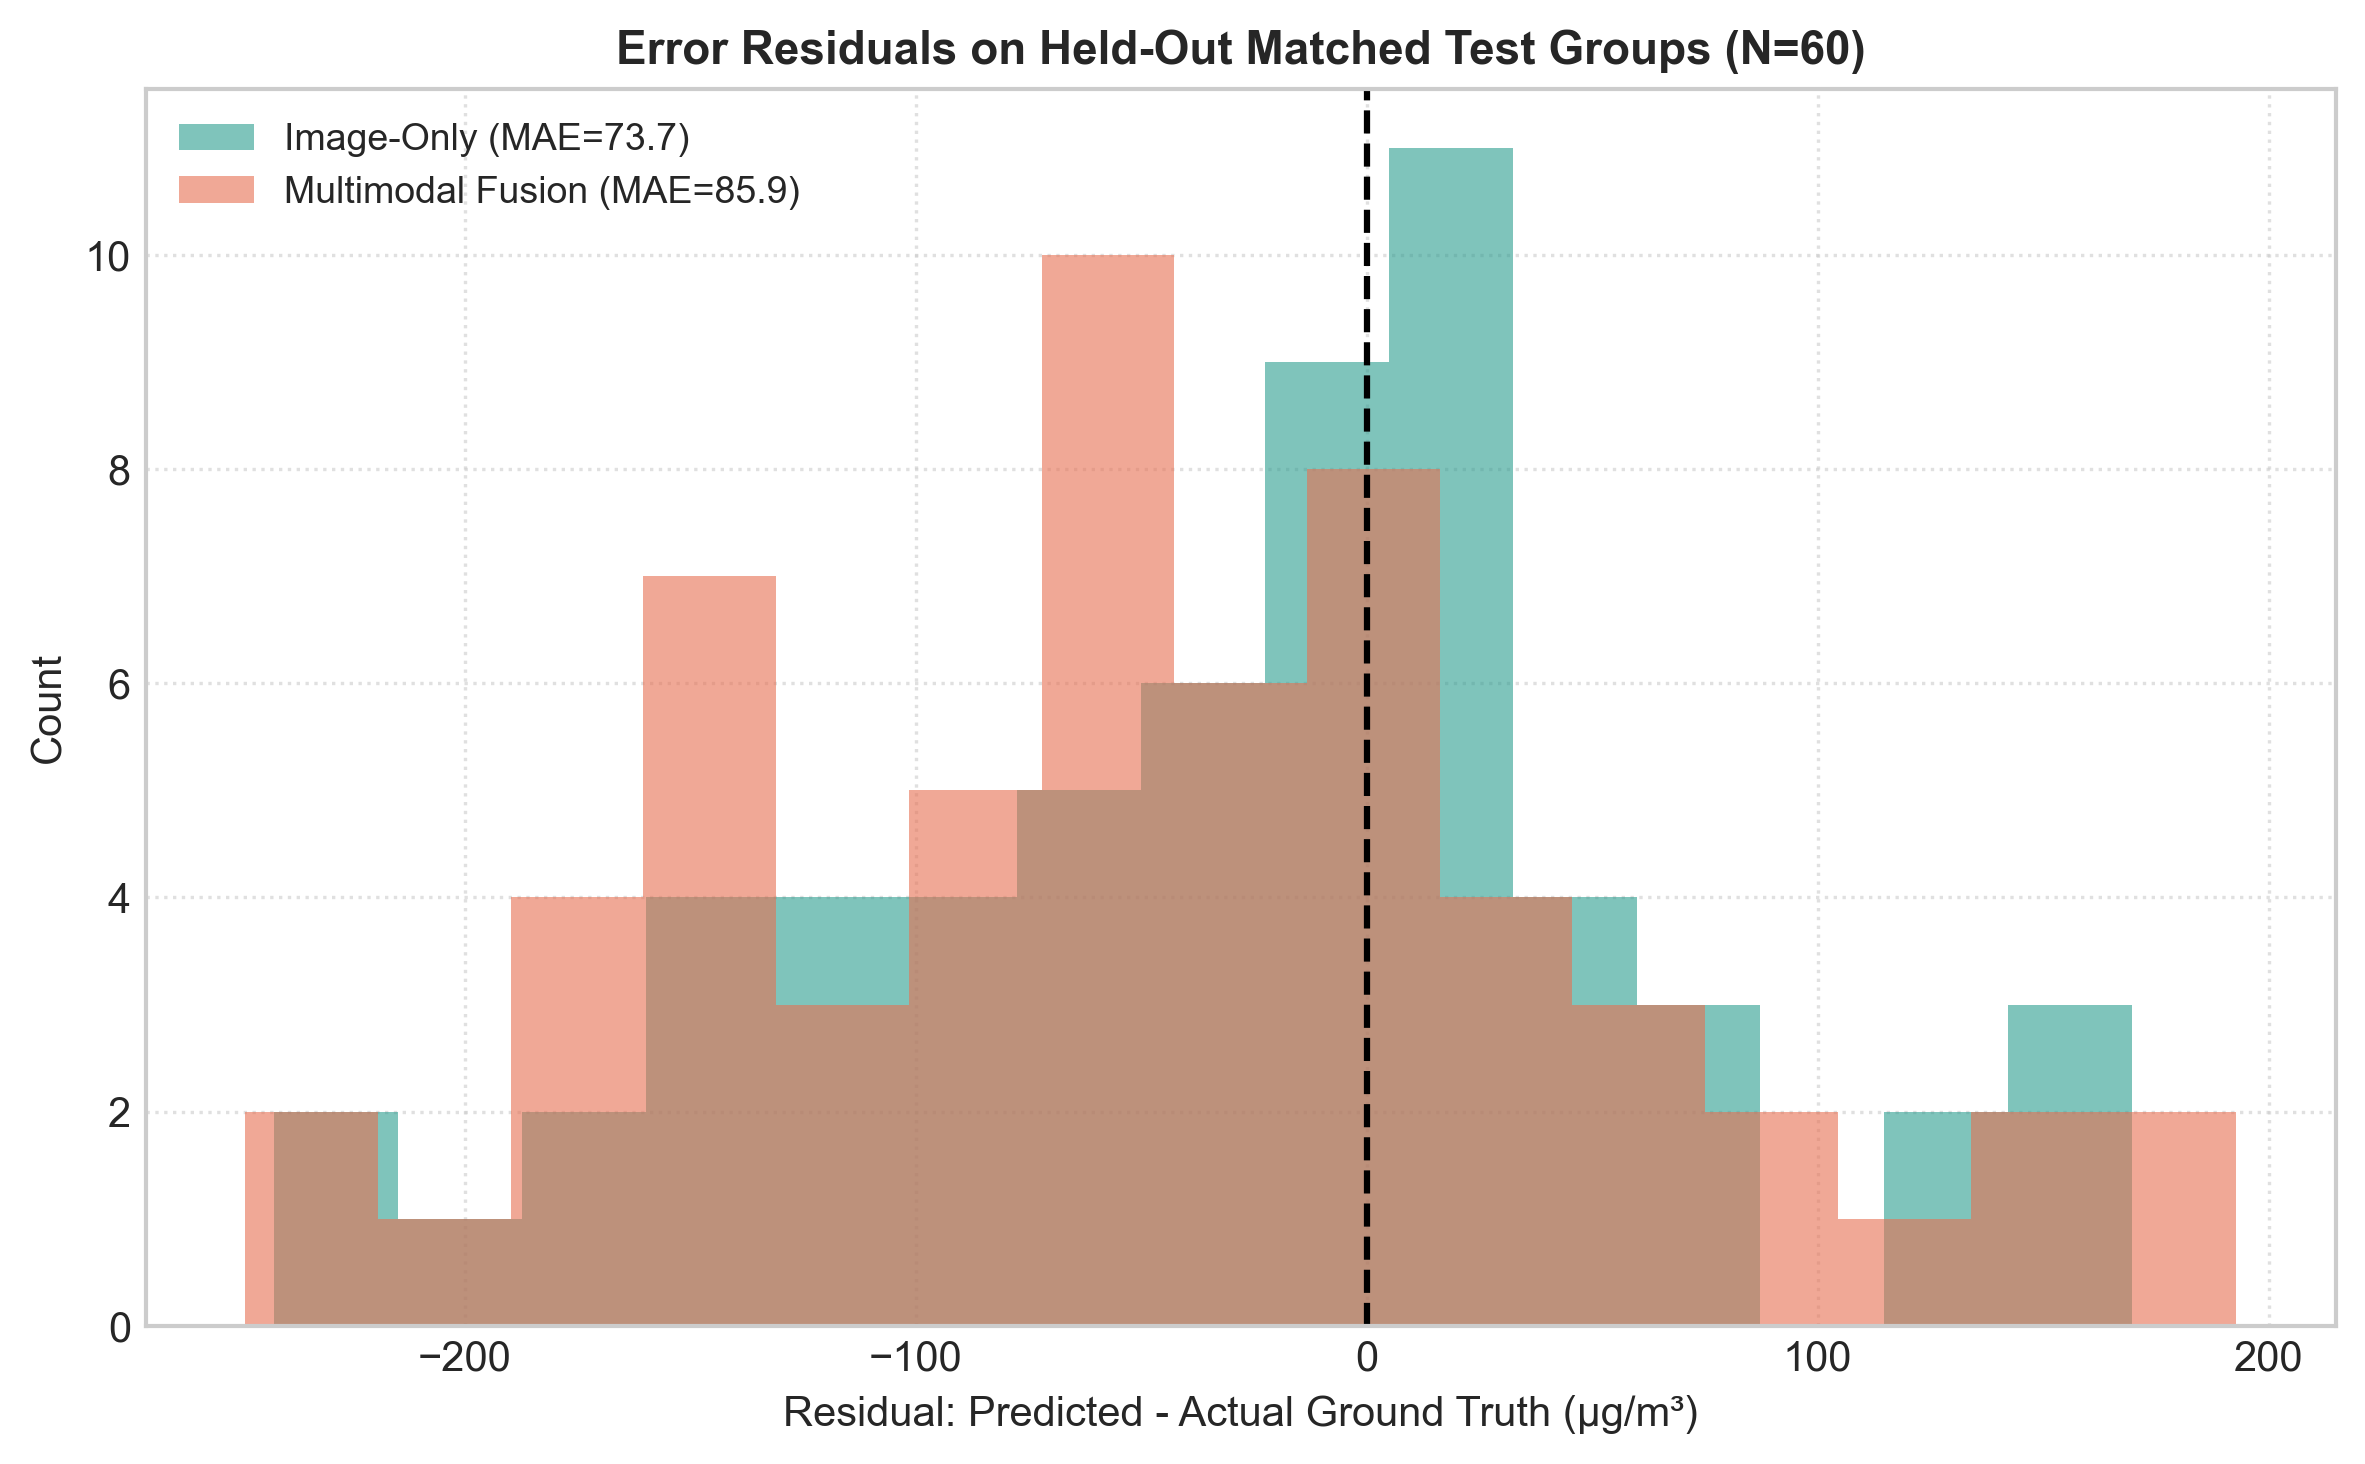
\includegraphics[width=\columnwidth]{matched_residual_distribution.png}
\caption{Distribution of prediction error residuals on the held-out matched test cohort ($N=60$ samples across 9 groups), comparing Image-Only and Multimodal Early Fusion.}
\label{fig:residuals}
\end{figure}

As illustrated in the residual distributions of Fig.~\ref{fig:residuals}, multimodal early fusion exhibits a broader error dispersion compared to image-only regression, driven by noise introduced by static daily meteorological variables across mismatched urban contexts.

\section{Limitations and Threats to Validity}
\begin{enumerate}
    \item \textbf{Lack of Fine-Grained Image Timestamps}: Public vision datasets often omit exact capture times, precluding sub-daily temporal alignment.
    \item \textbf{Spatial Displacement}: Matching images within 5 km assumes uniform air parcel composition, which is frequently violated in complex urban topographies with street-level canyons.
    \item \textbf{Extreme Pseudo-Replication}: High sample counts in raw manifests can mask tiny underlying group support (40\% of matches stemming from 2 days).
    \item \textbf{Label Provenance Divergence}: Web-scraped image labels exhibit severe positive calibration offsets (+70.74 $\mu\text{g/m}^3$) relative to certified federal monitors.
\end{enumerate}

\section{Conclusion and Future Work}
This work examined multimodal air quality prediction in Indian urban environments across 90 continuous stations, ERA5-Land meteorology, and outdoor imagery. The 2-layer numerical LSTM serves as a strong operational baseline for next-hour forecasting, while ResNet-50 provides an exploratory baseline for image-only estimation. However, rigorous feasibility auditing and controlled experiments prove that next-hour multimodal fusion is currently unsupported by opportunistic image datasets due to temporal asynchrony, small effective group counts ($N_{\text{groups}}=36$), and systematic calibration bias.

To realize effective multimodal air quality forecasting, future research must establish:
\begin{itemize}
    \item Collocated fixed camera networks mounted directly at ground monitoring stations recording synchronous hourly time-lapse images.
    \item Second-level EXIF timestamp synchronization with regulatory sensor data loggers.
    \item Radiometrically calibrated multi-spectral imaging to prevent optical saturation during severe smog episodes.
\end{itemize}

\bibliographystyle{IEEEtran}
\bibliography{references}

\end{document}
